\pdfoutput=1

\documentclass{article}

% Use the following line for the initial blind version submitted for review:
% \usepackage{icml2025}

% If accepted, instead use the following line for the camera-ready submission:
\usepackage[accepted]{icml2025}

% Recommended, but optional, packages for figures and better typesetting:
\usepackage{microtype}
\usepackage{subfigure}
\usepackage{natbib}
% \setcitestyle{numbers,square}
% \setcitestyle{authoryear}


% generic packages
% \usepackage[left=1in, right=1in, top=1in, bottom=1in]{geometry}
\usepackage[utf8]{inputenc}
\usepackage{amsmath,amsfonts}
\usepackage{amssymb}
\usepackage{graphicx}
\usepackage{tikz}
\usepackage{mathtools}
\usepackage{amsthm}
\usepackage{nccmath}
\usepackage{xspace}
\usepackage{xcolor}
\usepackage{booktabs}
\usepackage{array}
\usepackage{subcaption}
\usepackage{mathrsfs}
\definecolor{MyBlue}{rgb}{0.12, 0.12, 0.76}
\definecolor{MyPurple}{rgb}{0.8, 0.1, 0.8}
\definecolor{MyGreen}{rgb}{0.7, 0.1, 0.1}
\definecolor{MyRed}{rgb}{0.8, 0.1, 0.3}
\definecolor{MyYellow}{rgb}{0.7, 0.7, .1}
\definecolor{MyBlue2}{rgb}{0.1, 0.1, 0.6}
\definecolor{Color3}{HTML}{D62728}
\definecolor{Color1}{HTML}{0050C8}
\definecolor{Color2}{HTML}{4DAF4A}
\usepackage[colorlinks,allcolors=black]{hyperref}
\usepackage{pifont}% http://ctan.org/pkg/pifont
\newcommand{\cmark}{\ding{51}}
\newcommand{\xmark}{\ding{55}}



\usepackage[group-separator={,}]{siunitx}
\usepackage{url}
\usepackage{enumitem}
\usepackage{pdflscape}
\usepackage{verbatim}
\usepackage{arydshln}
\usepackage{multirow}
\usepackage{bigdelim}
\usepackage{stfloats}
\usepackage{pgfplots}
\usepackage{cleveref}
% \usepackage[capitalize,noabbrev]{cleveref}
\usepackage[font=small]{caption}
\newsavebox{\taxonomy}


\usetikzlibrary{shadows,arrows,decorations,decorations.shapes,backgrounds,shapes,snakes,automata,fit,petri,shapes.multipart,calc,positioning,shapes.geometric,graphs,graphs.standard,plotmarks,math,arrows.meta}
\usepackage{tikz-qtree}

% so I can restate theorems
\usepackage{thmtools}
\usepackage{thm-restate}

% Theorems
\theoremstyle{plain}
\newtheorem{theorem}{Theorem}[section]
\newtheorem{proposition}[theorem]{Proposition}
\newtheorem{lemma}[theorem]{Lemma}
\newtheorem{corollary}{Corollary}[theorem]
% \theoremstyle{definition}
\newtheorem{definition}[theorem]{Definition}
\newtheorem{assumption}[theorem]{Assumption}
\theoremstyle{remark}
\newtheorem{remark}[theorem]{Remark}

% Restate with same number, different text
    \newtheoremstyle{TheoremNum}
        {\topsep}{\topsep}              %%% space between body and thm
        {\itshape}                      %%% Thm body font
        {}                              %%% Indent amount (empty = no indent)
        {\bfseries}                     %%% Thm head font
        {.}                             %%% Punctuation after thm head
        { }                             %%% Space after thm head
        {\thmname{#1}\thmnote{ \bfseries #3}}%%% Thm head spec
    \theoremstyle{TheoremNum}
    \newtheorem{theoremNumbered}{Theorem}





% To define a Construction environment
\usepackage{newfloat}
\DeclareFloatingEnvironment[
    fileext=los,
    listname={List of Constructions},
    name=Construction,
    placement=Htbhp,
]{construction}

%Pseudocode stuff
% \usepackage{algorithm}
% \usepackage{algpseudocode}
% \usepackage{algorithmicx}
% \renewcommand{\algorithmicforall}{\textbf{for each}} % ``for all'' -->``for each''
% \let\oldReturn\Return
% \renewcommand{\Return}{\state\oldReturn}
% \algtext*{EndWhile}% Remove "end while" text
% \algtext*{EndIf}
% \algtext*{EndForAll}
% \algtext*{EndFor}
% \algtext*{EndFunction}
\renewcommand{\algorithmicendfor}{\vspace{-1.2em}}%
\renewcommand{\algorithmicendif}{\vspace{-1.2em}}%

\DeclarePairedDelimiter{\ceil}{\lceil}{\rceil}
\DeclareMathOperator*{\argmax}{arg\,max}
\DeclareMathOperator*{\E}{\mathbb{E}}
\DeclareMathOperator*{\argmin}{arg\,min}
\DeclareMathOperator*{\len}{len}
\DeclareMathOperator*{\conv}{conv}
\DeclareMathOperator*{\vol}{vol}
\DeclareMathOperator*{\diam}{diam}


\newcommand\bbr{\mathbb{R}}
\newcommand\bbrpos{\mathbb{R}_{\ge 0}}
\newcommand\bbrspos{\mathbb{R}_{> 0}}
\newcommand\bbn{\mathbb{N}}
\newcommand\ep{\varepsilon}
\newcommand\hata{\hat{a}}
\renewcommand{\d}[1]{\ensuremath{\operatorname{d}\!{#1}}}
\newcommand\X{\mathcal{X}}
\newcommand\smola{\boldsymbol{a}}
\newcommand\smols{\boldsymbol{s}}
\newcommand\s{\mathcal{S}}
\newcommand\sm{\boldsymbol{s^m}}
\newcommand\A{\mathcal{A}}
\newcommand\bfone{\boldsymbol{1}}
\newcommand\norm[1]{||#1||}
\newcommand\tv[1]{||#1||_{TV}}
\newcommand\bfmu{\boldsymbol{\mu}}
\newcommand\muprime{\boldsymbol{\mu'}}
\newcommand\M{\mathcal{M}}
\newcommand\bars{\bar{s}}
\newcommand\rac{R_T^{AC}}
\newcommand{\spr}{\mathcal{S'}}
\newcommand{\mpr}{\mathcal{M'}}
\newcommand\apr{\mathcal{A'}}
\newcommand\U{\mathcal{U}}
\newcommand\tilpi{\tilde{\Pi}}
\newcommand\stilpi{\tilde{\pi}}
\newcommand\D{\mathcal{D}}
\newcommand\B{\mathcal{B}}

\newcommand\stuart[1]{{\color{purple}Stuart: #1}}
\newcommand\juan[1]{{\color{blue}Juan: #1}}
\newcommand\todo[1]{{\color{red}TODO: #1}}
% \renewcommand\todo[1]{}

% \title{Asking for Help Enables Safety Guarantees Without Sacrificing Effectiveness}

% \author{Benjamin Plaut\thanks{Corresponding author} \\
% UC Berkeley \\
% \texttt{plaut@berkeley.edu}
% \and Juan Liévano-Karim \\
% UC Berkeley \\
% \texttt{jp.lievano10@uniandes.edu.co}
% \and Stuart Russell \\
% UC Berkeley \\
% \texttt{russell@berkeley.edu}
% }

% \author{Anonymous authors}


\date{}

\icmltitlerunning{Asking for Help Enables Safety Guarantees Without Sacrificing Effectiveness}

\begin{document}

\twocolumn[
\icmltitle{Asking for Help Enables Safety Guarantees\\ Without Sacrificing Effectiveness}

% \maketitle

\icmlsetsymbol{equal}{*}

\begin{icmlauthorlist}
\icmlauthor{Benjamin Plaut}{ucb}
\icmlauthor{Juan Liévano-Karim}{ucb}
\icmlauthor{Stuart Russell}{ucb}
\end{icmlauthorlist}

\icmlaffiliation{ucb}{University of California, Berkeley}

\icmlcorrespondingauthor{Benjamin Plaut}{plaut@berkeley.edu}

% You may provide any keywords that you
% find helpful for describing your paper; these are used to populate
% the "keywords" metadata in the PDF but will not be shown in the document
\icmlkeywords{safe RL,asking for help,irreversibility,regret}

\vskip 0.3in
]

\printAffiliationsAndNotice{}

\begin{abstract}
Retrieval-Augmented Generation (RAG) is often used with Large Language Models (LLMs) to infuse domain knowledge or user-specific information. In RAG, given a user query, a retriever extracts chunks of relevant text from a knowledge base. These chunks are sent to an LLM as part of the input prompt. Typically, any given chunk is repeatedly retrieved across user questions. However, currently, for every question, attention-layers in LLMs fully compute the key values (KVs) repeatedly for the input chunks, as state-of-the-art methods cannot reuse KV-caches when chunks appear at arbitrary locations with arbitrary contexts. Naive reuse leads to output quality degradation.  This leads to potentially redundant computations on expensive GPUs and increases latency. In this work, we propose \sys, a system for managing and reusing precomputed KVs corresponding to the text chunks (we call \textit{chunk-caches}) in RAG-based systems. We present how to identify \hl{\textit{chunk-caches} that are reusable}, how to efficiently perform a small fraction of recomputation to \textit{fix} the cache to maintain output quality, and how to efficiently store and evict \textit{chunk-caches} in the hardware for maximizing reuse while masking any overheads. With real production workloads as well as synthetic datasets, we show that \sys reduces redundant computation by \textbf{51\%} over SOTA prefix-caching and \textbf{75\%} over full recomputation.
\hl{Additionally, with continuous batching on a real production workload, we get a \textbf{1.6$\times$} speedup in throughput and a \textbf{2$\times$} reduction in end-to-end response latency over prefix-caching while maintaining quality, for both the \llama-3-8B and \llama-3-70B models. 
}
\end{abstract}






\section{Introduction}
\label{sec:intro}

\begin{figure*}[tb]
    \centering
    \includegraphics[width=0.848\linewidth]{figs/circuitnn.pdf} 
    \caption{Illustration of differentiable CircuitNN. CircuitNN is designed based on differentiable NAND gates. After DAS is guided by PI and PO pairs of the truth table, CircuitNN can get the precise circuit architecture logic equivalent to the truth table.}
    \label{fig:circuitnn}
\end{figure*}

% 1. Describe the importance of logic synthesis
% 2. Existing Problems
% (a) Neural Architecture Search: Unstable, Predefined Setting, etc.
% (b) Circuit Generation: Probabilistic Model, Logic Equivalence

With the rapid advancement of technology, the scale of integrated circuits (ICs) has expanded exponentially. 
This expansion has introduced significant challenges in chip manufacturing, particularly concerning power and area metrics.
A primary objective in IC design is achieving the same circuit function with fewer transistors, thereby reducing power usage and area occupancy.

Logic synthesis~\cite{hachtel2005logicsynth}, a critical step in electronic design automation (EDA), transforms behavioral-level circuit designs into optimized gate-level circuits, ultimately yielding the final IC layout. 
The primary goal of logic synthesis is to identify the physical implementation with the fewest gates for a given circuit function. 
This task constitutes a challenging NP-hard combinatorial optimization problem. 
Current logic synthesis tools~\cite{brayton2010abc, wolf2013yosys} rely on human-designed heuristics, often leading to sub-optimal outcomes.

Differentiable architecture search (DAS) techniques~\cite{liu2018darts, chu2020darts} offer novel perspectives on addressing challenges in this problem.
Circuit functions can be represented through truth tables, which map binary inputs to their corresponding outputs. 
Truth tables provide a precise representation of input-output relationships, ensuring the design of functionally equivalent circuits.
Inspired by this, researchers~\cite{deepmind2024ai4sys, wang2024tnet} have begun exploring the application of DAS to synthesize circuits directly from truth tables.
Specifically, \citet{deepmind2024ai4sys} proposed CircuitNN, a framework that learns differentiable connection structures with logic gates, enabling the automatic generation of logic circuits from truth tables.
This approach significantly reduces the complexity of traditional circuit generation. 
Building on this, \citet{wang2024tnet} introduced T-Net, a triangle-shaped variant of CircuitNN, incorporating regularization techniques to enhance the efficiency of DAS.

Despite these advancements, several challenges remain. 
The computational complexity of DAS grows quadratically with the number of gates, posing scalability issues.
Although triangle-shaped architecture~\cite{wang2024tnet} partially mitigates this problem, redundancy persists. 
%Additionally, DAS is susceptible to converging to local optima, limiting the ability to search architectures that satisfy the given truth tables~\cite{liu2018darts}. 
%Furthermore, hyperparameters (network depth and layer width) require extensive searches, introducing complexity and prolonging the synthesis process. 
Additionally, DAS is susceptible to converging to local optima~\cite{liu2018darts} and hyperparameters (network depth and layer width) require extensive searches. 
The challenges arise from the vast search space in DAS. 
% Even with predefined settings for CircuitNN, finding a configuration that meets the truth table requires extensive trial and error during the DAS process. 
Intuitively, limiting the search space through predefined parameters (network depth, gates per layer, and connection probabilities) can significantly reduce the complexity.

Recent advances~\cite{openai2023gpt4, abramson2024alphafold3, esser2024sd3, li2024mar} in conditional generative models have demonstrated remarkable performance across language, vision, and graph generation tasks. 
Motivated by these developments, we propose a novel approach to circuit generation that generates preliminary circuit structures to guide DAS in generating refined circuits matching specified truth tables. 
Firstly, we introduce CircuitVQ, a tokenizer with a discrete codebook for circuit tokenization. 
Built upon our Circuit AutoEncoder framework~\cite{hou2022graphmae,li2023maskgae,wu2025mgvga}, CircuitVQ is trained through a circuit reconstruction task. 
Specifically, the CircuitVQ encoder encodes input circuits into discrete tokens using a learnable codebook, while the decoder reconstructs the circuit adjacency matrix based on these tokens.
Subsequently, the CircuitVQ encoder serves as a circuit tokenizer for CircuitAR pretraining, which employs a masked autoregressive modeling paradigm~\cite{chang2022maskgit, li2023mage}. 
In this process, the discrete codes function as supervision signals. 
After training, CircuitAR can generate discrete tokens progressively, which can be decoded into initial circuit structures by the decoder of the CircuitVQ. 
These prior insights can guide DAS in producing refined circuits that match the target truth tables precisely.

Our key contributions can be summarized as follows:
\begin{itemize}
\item We introduce CircuitVQ, a circuit tokenizer that facilitates graph autoregressive modeling for circuit generation, based on our Circuit AutoEncoder framework;
\item Develop CircuitAR, a model trained using masked autoregressive modeling, which generates initial circuit structures conditioned on given truth tables;
\item Propose a refinement framework that integrates differentiable architecture search to produce functionally equivalent circuits guided by target truth tables;
\item Comprehensive experiments demonstrating the scalability and capability emergence of our CircuitAR and the superior performance of the proposed circuit generation approach.
\end{itemize}

% Motivation
% (a) Diffusion (Vision, Graph), Autoregressive (Language, Vision)
% (b) Circuit Generation for Predefined Setting
% (c) Neural Architecture Search for Strict Logic Equivalence

% Contribution
% (a) Circuit Tokenizer (new transformer arch, training strategy)
% (b) CircuitAR (train and gen strategies, post-ar strategy)
% (c) Extensive Evaluation including BitD (Bit Distance) for Scalability


\section{Related Work}
% \subsection{Vision Language Model}
% 시각장애인에서 상황을 설명할 DB가 없으니 만들었다. 그리고 이를 VLM에 튜닝했다.
\subsection{Technical approaches for assisting the visually-impaired}


\subsection{Datasets for visual instruction tuning}


To illustrate equilibria and dynamics of performative prediction games, we focus on a scenario in which a \emph{duopoly} of mortgage companies, i.e. banks, compete to sell loans to customers.

\paragraph{Customer Model:} In our game, each bank is trying to attract customers from a given population $\mathcal{P}$. We model this population as comprised of individuals with a single-dimensional type: we denote individual $j$'s type as $y_j \in [0,1]$. For simplicity, we assume that \(y\) represents the customer’s probability of repaying the loan\footnote{In practice, a customer's (normalized) credit score can be interpreted as a noisy observation of $y_j$. This also corresponds to credit scores being \emph{calibrated}.}, i.e., $y_j := \P[Y_j = 1]$, where $Y_j$ is a random variable such that $Y_j = 0$ means that $j$ defaults on their loan, and $Y_j = 1$ means they repay their loan. Customer types in the population are drawn from a known distribution $D_y$ supported on $[0,1]$. 

\paragraph{Game between Banks:} Each Bank \(i \in \{1, 2\}\) selects two parameters \( (\tau_i, \gamma_i) := \theta_i\), where:
\begin{itemize}
    \item \(\tau_i \in \{\tau_l,\tau_h\}\) is the credit score threshold for approving a customer\footnote{We restrict the bank to only pick between two thresholds, $\tau_l$ and $\tau_h$. However, we highlight how our results are affected when we expand the strategy space to $n > 2$ actions in our experiments of Appendix \ref{app:3gamma}.}. Specifically, a customer $j$ with credit score \(y_j\) is approved by Bank $i$ if and only if \(y_j \geq \tau_i\);
    \item \(\gamma_i \in \{\gamma_l, \gamma_h\}\) is the interest rate offered to approved customers.
\end{itemize}
We denote as shorthand the space of allowable thresholds by $\Gamma := [0,1]$ and allowable interests rates by $\Lambda := [0,1]$. %The latter is set without loss of generality---we simply normalize the rates to be at most $1$. 
% {\color{red} Vidya: just thinking about this but is it natural to restrict interest rate to $1$? I don't think it would affect the equilibrium structure of the game but theoretically I think the interest rate could be anything in $[0,\infty)$.} {\color{green} Guanghui: Could we say something like this is without loss of generality} \gua{changed.}\juba{I think we repeated this twice, the next sentence already had this}
The loan amount is normalized to $1$ in the entire paper, without loss of generality; in this case, if a customer chooses Bank $i$, and the customer is approved by the bank at an interest rate of $\gamma_i$, the expected utility for the bank is equal to
\[
(1+\gamma_i)\cdot \P[Y_i = 1]-\P[Y_i = 0] = (1+\gamma_i)y_i-(1-y_i).
\]


%In practice, the credit score \(y\) serves as a noisy observation of the true likelihood of the customer's repayment. 

\paragraph{Banks' Utilities:} For given parameter choices \(\theta_1 = (\tau_1, \gamma_1)\) by Bank 1 and \(\theta_2 = (\tau_2, \gamma_2)\) by Bank 2, a \emph{rational} customer with credit score $y$ acts as follows:

\begin{enumerate}
    \item \textbf{Qualified for a single bank}: 
        \begin{itemize}
        \item If \(\tau_1 \leq y < \tau_2\), the customer goes to Bank 1, as the score qualifies for Bank 1 but not Bank 2. Conversely, if \(\tau_2 \leq y < \tau_1\), the customer chooses Bank 2.
    \end{itemize}
    \item \textbf{Qualified for both banks}:
     \begin{itemize}
        \item If \(\tau_1, \tau_2 \leq y\) and \(\gamma_1 < \gamma_2\), the customer selects Bank 1 for its lower interest rate. Conversely, if \(\gamma_1 > \gamma_2\), the customer chooses Bank 2.
        \item If \(\gamma_1 = \gamma_2\), the customer picks each bank with probability $1/2$. 
    \end{itemize}
    \item \textbf{Unqualified for both banks}:
    \begin{itemize}
        \item If \(y < \tau_1\) and \(y < \tau_2\), the customer is rejected by both banks.
    \end{itemize}
\end{enumerate}

The expected reward for Bank 1, denoted as \(u_1(\theta_1, \theta_2)\), can then be expressed as:
\begin{align}\label{eq:utility}
    u_1(\theta_1, \theta_2) 
    &=  \mathbb{E}_{y \sim D_y} \left[ \mathbb{I}\{\underbrace{\tau_1 \leq y < \tau_2 \ \cup \ (\tau_1, \tau_2 \leq y \ \cap \ \gamma_1 < \gamma_2)}_{\text{accepted by Bank 1}}\} \cdot \big((1+\gamma_1)y - (1-y)\big) \right] \nonumber\\
    & + \frac{1}{2} \mathbb{E}_{y \sim D_y} \left[ \mathbb{I}\{\underbrace{\tau_1, \tau_2 \leq y \ \cap \ \gamma_1 = \gamma_2}_{\text{accepted by both Banks}}\} \cdot \big((1+\gamma_1)y - (1-y)\big) \right].
\end{align}
Note that the problem is \emph{symmetric}, i.e., the utility function for Bank 2 can be derived by swapping the roles of \(\theta_1\) and \(\theta_2\). I.e., $u_2(\theta_1, \theta_2) = u_1(\theta_2, \theta_1)$. 

% If a bank only attracts customers between thresholds $\tau_a$ and $\tau_b$, for $\tau_a<\tau_b$, we call $[\tau_a,\tau_b]$ the \emph{threshold} range for that bank. For example, if Bank $1$ sets a threshold of $\tau_1$, Bank $2$ a threshold of $\tau_2 > \tau_1$, and $\gamma_1 > \gamma_2$, then Bank 1 has a threshold range of $[\tau_1,\tau_2]$, while bank $2$ has a threshold range of $[\tau_2,1]$.
% Note that the parameters set by \emph{both} banks, i.e. $(\theta_1,\theta_2)$ both influence the threshold range for each of Bank 1 and 2.  If $\tau_1>\tau_2$, $\gamma_1>\gamma_2$, then $\tau_a>\tau_b$, and the bank does not attract any customers. 
% {\color{red} is it possible for $\tau_a > \tau_b$, leading to the bank never attracting customers?} \gua{if $\gamma_1>\gamma_2$, $\tau_1>\tau_2$, then it gets no customer. I think it also makes sense.}\juba{I think we said we wanted to delete the discussion of the threshold range, no?}

% \noindent \textbf{Discrete Model}   
% We now present the discrete version of our model, where the interest rates and thresholds are selected from finite sets \(\Gamma\) and \(\Lambda\), respectively, with $\tau\in[0,1], \gamma\in[0,1]$,  for all $\tau\in\Lambda$ and $\gamma\in\Gamma$, \(|\Gamma| = n\) and \(|\Lambda| = m\). Let \(p_1, p_2 \in \Delta(\Gamma \times \Lambda)\) represent the mixed strategies of the two banks, where \(\Delta(\Gamma \times \Lambda)\) denotes the set of probability distributions over the discrete decision space \(\Gamma \times \Lambda\).


% \begin{Remark}
%    Note that our proposed problem can be reformulated as a standard multi-player performative prediction problem \citep{narang2023multiplayer}. However, in our problem, the data distribution faced by each learner breaks the Lipschitzness assumption of previous work~\citep{hardt2023performative,narang2023multiplayer}. A small modification in one of the learner's thresholds can completely change how demand is allocated across both learners, as is often the case in Bertrand-style games. 
% \end{Remark} 

% \gua{I made some changes to Remark 1, please have a look}
\begin{Remark}
   Previous works in multi-learner performative prediction~\citep{narang2023multiplayer} resort to an insensitivity assumption, i.e., the data distribution faced by each player can only changes slightly when the parameters also change slightly; formally, the data distribution faced by each player is Lipschitz in their decisions. This is immediately not true in our setting: the bank slightly changing its parameters can completely changes the demand distribution of customers it faces. Intuitively, this is because of Bertrand-competition-style effects, where if two banks have similar rates, one bank that lowers their rate by a small amount suddenly captures the entire customer demand that is eligible for that rate.%\juba{made further light edits adding intuition}
   
   In Appendix \ref{Appendix:refumulation}, we discuss this problem more carefully by reformulating our problem in the standard multi-learner performative prediction form given by~\citep{narang2023multiplayer}. We show the distribution is not Lipschitz with respect to the parameters, and thus does not satisfy the insensitivity assumption. 
%Prior work~\citep{hardt2023performative,narang2023multiplayer} showed that, for a general multi-agent performative prediction framework to work, insensitivity assumptions are needed: in the \textbf{worst case}, they can construct settings where the insensitivity assumption does not hold and simple dynamics do not converge anymore. We add nuance to this picture. We will show that our dynamics often converge, even absent insensitivity assumptions, highlighting that while the impossibility results of previous work hold in the worst case, they may not hold in the ``average case'' and especially not in problems motivated by applications. In particular, we will show convergence to a variety of equilibria of our game, and often to symmetric Nash equilibria where insensitivity is immediately violated.
     
\end{Remark}



% \paragraph{Relationship to Performative Prediction} A central point of our work is to highlight that \textcolor{red}{needs writing from intro}. We highlight how our work specifically ties to ``Performative Prediction'' below:


%\textcolor{red}{needs a definition environment}



%Here, \(\E_{\theta_1, \theta_2}\) represents the expected utility of the banks over their respective strategies \((\theta_1, \theta_2)\). These inequalities ensure that neither bank can unilaterally improve its expected utility by deviating from its mixed strategy in the equilibrium.



%and  for all $\tau\in\Gamma$, we have $\tau\in\Lambda$, $(\tau,\gamma)\in[0,1]^2$. Let $\Gamma\times\Lambda$
%In this paper, we focus on the most fundamental case, where there are two choices for each parameter: $0\leq\tau_{\ell}<\tau_{h}\leq 1$, and $0\leq \gamma_{\ell}< \gamma_{h}\leq 1$. In this case, the utility for each pair of decisions forms a $4\times4$ matrix (given in Table \ref{tab:my-table}). We consider the canonical case where $\tau_{\ell}=\frac{1}{2+\gamma_{h}}$, and $\tau_{h}=\frac{1}{2+\gamma_{\ell}}.$ Note that these are natural choices for the thresholds, in the sense that, if there is only one bank and the interest rate is set to be $\gamma$, then $\frac{1}{2+\gamma}$ is the optimal threshold corresponding to the fixed $\gamma$.


%and the thresholds are chosen in $\Lambda=\{\tau^{(1)},\dots,\tau^{(m)}\}$. Here, we only assume that, for each $\gamma\in\Gamma$, there at least exist one $\tau\in\Lambda$ such that $f(\gamma,\tau,1)>0$. Note that this is a very minor assumption, in the sense that, if for a $\gamma$ such that $f(\gamma,\tau,1)<0$ for all $\tau\in\Lambda$, then adopting this decision will lead to negative utility regardless of the opponent's decision, and thus is not an interesting case. 

%\textcolor{red}{The model section is missing the dynamic version of the game. We should clearly define the one-shot and the dynamic game}
% we only considered one-shot case in our paper





\begin{table*}[b!]
\centering
\caption{The key differences between our model and that of \citet{plaut_avoiding_2024}.}
\begin{tabular}{p{0.18\textwidth} p{0.36\textwidth} p{0.36\textwidth}}
\toprule
\textbf{Aspect} & \textbf{Our model} & \textbf{Model of \citet{plaut_avoiding_2024}} \\
\midrule
Conceptual goal & Maximize reward and avoid catastrophe & Avoid catastrophe only \\
% \midrule
% Reward meaning & Typical meaning & Chance of no catastrophe that round\\
\midrule
Objective & Sum of payoffs & Product of payoffs \\
\midrule
Regret definition & Agent and mentor evaluated on $\smols,\sm$ & Agent and mentor both evaluated on $\smols$ \\
\midrule
Desired regret & Sublinear in $T$ & Subconstant in $T$ \\
% \midrule
% Source of next state & MDP transition function & Adversary \\
% \midrule
% Smoothness & $\sigma$-smooth transition function & $\sigma$-smooth adversary \\
\bottomrule
\end{tabular}
\label{tab:model-comparison}
\end{table*}

\section{Avoiding catastrophe in \citet{plaut_avoiding_2024} and in MDPs}\label{sec:ac-overview}

Since our main result is a reduction to \citet{plaut_avoiding_2024}, we first describe their work. This section also serves to establish the novelty of our contribution in relation to \citet{plaut_avoiding_2024}. Some technical details are deferred to Appendix~\ref{sec:ac-full}.

Our model and that of \citet{plaut_avoiding_2024} are quite similar, so their model is perhaps best understood through comparison with our model. In place of $r$, they consider a sequence of reward functions $\bfmu = (\mu_1,\dots,\mu_T)$, where $\mu_t: \s\times\A\to[0,1]$ represents the probability of avoiding catastrophe at time $t$ (conditioned on no prior catastrophe). They aim to maximize the product of rewards from $\bfmu$, which is equal to the overall chance of avoiding catastrophe by the chain rule of probability. They also make a local generalization assumption: letting $\mu_t^m(s) = \mu_t(s, \pi^m(s))$ for brevity, we say that $\bfmu$ satisfies local generalization if $|\mu_t^m(s) - \mu_t(s, \pi^m(s'))| \le L\norm{s - s'}$ for all $s, s'\in \s$ and $t \in [T]$.


% \emph{Regret definition.} We evaluate the agent and mentor on their respective state sequences (as determined by their respective actions and the transition kernel). Instead, \citet{plaut_avoiding_2024} assume that a single state sequence is provided by an adversary\footnote{Their adversary can be adaptive: the choice of $s_t$ and $\mu_t$ can depend on the events of prior time steps.} and evaluate both the agent and the mentor on that same sequence. 

% \emph{Desired regret.} Instead of sublinear regret, \citet{plaut_avoiding_2024} demand \emph{subconstant} regret. That is, the total (not average) regret should go to 0 as $T \to\infty$. However, we will see that subconstant regret in their setting is of the same ``difficulty'' as sublinear regret in our setting (\Cref{sec:ac-mdp}).



\Cref{tab:model-comparison} summarizes the differences between our models. Formally, we arrive at \Cref{def:ac}:

\begin{restatable}{definition}{defAC}
\label{def:ac}
Let $\rac = \sup_{\M, \pi^m,\bfmu} \E[\sum_{t=1}^T \mu_t^m(s_t) - \sum_{t=1}^T \mu_t(s_t, a_t)]$, where the supremum ranges over all $\bfmu$ satisfying local generalization. Then an algorithm \emph{avoids catastrophe} if $Q_T \in o(T)$ and $\lim_{T\to\infty} \rac = 0$.\looseness=-1
\end{restatable}

\Cref{def:ac} was intended by \citet{plaut_avoiding_2024} to represent avoiding catastrophe. This interpretation can be debated, but ultimately we primarily use \Cref{def:ac} as a mathematical tool for our main goal: a no-regret algorithm for general MDPs. As such, what really matters is that \citet{plaut_avoiding_2024} give an algorithm satisfying \Cref{def:ac}.

% First, instead of evaluating the mentor on $\sm$ and the agent on $\smols$, \Cref{def:ac} evaluates both on $\smols$: this makes the problem easier. On the flip side, \Cref{def:ac} demands subconstant regret instead of sublinear regret, which makes the problem harder.  problem is not obviously easier or harder than our problem

% There are two subtleties in \Cref{def:ac}. 

Before stating the relevant lemma, we discuss two subtleties of \Cref{def:ac}. First, \citet{plaut_avoiding_2024} assume that the agent never observes $\mu_t(s_t,a_t)$ and only learns from mentor queries. Thus for fixed $\M$ and $\pi^m$, the choice of $\bfmu$ does not affect the behavior of the algorithm. As a result, \Cref{def:ac} in effect requires that for any $\M$ and $\pi^m$, the algorithm satisfies $\E[\sum_{t=1}^T \mu_t^m(s_t) - \sum_{t=1}^T \mu_t(s_t, a_t)] \le \rac$ \emph{simultaneously} for every $\bfmu$ satisfying local generalization. This enables us to use multiple choices of $\bfmu$ in our reduction.

Second, the reader may notice that \Cref{def:ac} involves the sum of rewards, while we stated previously that \citet{plaut_avoiding_2024} study the products of rewards. However, in this particular context, the sum and product formulations are roughly equivalent (\Cref{prop:sum-prod}).\footnote{This is mostly due to the approximation $1+x \approx e^x$ for $x \approx 0$.} Indeed, \citet{plaut_avoiding_2024} also include additive versions of all of their regret bounds. We use their additive bounds since those are more convenient for us. Specifically, they prove the following:\looseness=-1

% \footnote{Although \Cref{lem:ac-regret} assumes binary actions, \citet{plaut_avoiding_2024} also provide a version for any finite number of actions (Algorithm 3 and Theorem C.1 in their paper). Our result applies equally to that version -- indeed, our result is a general reduction -- but the many-action version requires more terminology to state, so we have chosen to only include the binary-action version here.}
\begin{lemma}[Theorems 5.2 and 5.3 in \citet{plaut_avoiding_2024}]
\label{lem:ac-regret}
    Let $\A = \{0,1\}$. Assume $\pi^m \in \Pi$ and either (1) $\Pi$ has finite VC dimension $d$ and $P$ is $\sigma$-smooth or (2) $\Pi$ has finite Littlestone dimension $d$.\footnote{The second case does not assume $\sigma$-smoothness, so the regret and query bounds in that case do not actually depend on $\sigma$. However, for brevity, we just write a single set of bounds.} Then Algorithm 1 in \citet{plaut_avoiding_2024} avoids catastrophe (\Cref{def:ac}) with
    % $Q_T \in  O(T^\frac{4n+1}{4n+2}(\frac{d}{\sigma} \log T + \diam(\smols)^n))$ and $\rac \in O(\frac{dL}{\sigma}T^\frac{-1}{2n+1} \log T)$.
\begin{align*}
Q_T \in&\  O\left(T^\frac{4n+1}{4n+2}\Big(\frac{d}{\sigma} \log T + \diam(\smols)^n\Big)\right)\\
\rac \in&\ O\left(\frac{dL}{\sigma}T^\frac{-1}{2n+1} \log T\right)
\end{align*}
\end{lemma}

Their algorithm has several beneficial properties beyond the regret and query bounds: it can handle an unbounded state space (the number of queries scales with the diameter of observed states), it does not need to know $L$, and it does not need to know how states are encoded in $\bbr^n$. See Appendix~\ref{sec:ac-full} for pseudocode for their algorithm.

Although \Cref{lem:ac-regret} requires $\A = \{0,1\}$, \citet{plaut_avoiding_2024} also provide a version for any finite number of actions (Algorithm 3 and Theorem C.1 in their paper). Our reduction applies equally to that version, but the many-action version requires more terminology to state, so we have chosen to only include the binary-action version here.


Lastly, although this does not directly bear on our results, it is worth mentioning that \citet{plaut_avoiding_2024} also prove a negative result: without the assumptions of \Cref{lem:ac-regret}, no algorithm satisfies both $Q_T \in o(T)$ and $\rac \in o(1)$, even for a simple environment: $\s = [0,1]$, i.i.d. states, and $\bfmu$ does not vary between time steps. We can expect this negative result to apply to our setting too, since obtaining high reward requires avoiding catastrophe. But what does ``catastrophe'' mean in an MDP?\looseness=-1

\textbf{Catastrophe in MDPs.} In contrast to the model of \citet{plaut_avoiding_2024}, MDPs do not directly model catastrophe in an objective function. Instead, notions of catastrophe arise naturally through the environment dynamics: for example, the agent might get stuck in an inescapable zero-reward state.\looseness=-1

\begin{figure*}[b]
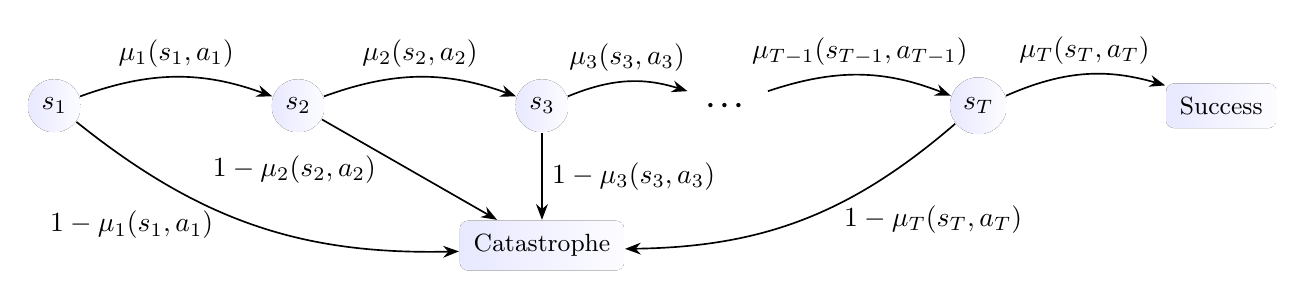
\begin{tikzpicture}[>={Stealth[scale=1]}, 
    semithick, 
    node distance=2.4cm, 
    auto, 
    state/.style={align=center,circle,inner sep=3pt,path picture={\fill[left color=blue!9, right color=blue!1] (path picture bounding box.south west) rectangle (path picture bounding box.north east);}}
    ]
    % Nodes
    \node[state] (S1) {$s_1$};
    \node[state, right=of S1] (S2) {$s_2$};
    \node[state, right=of S2] (S3) {$s_3$};
    \node[right=1.5cm of S3, minimum width=1 cm] (dots) {$\boldsymbol{\cdots}$};
    \node[state, right=2.3cm of dots] (ST) {$s_T$};
    \node[state, rectangle, rounded corners=3pt, below=1.1cm of S3, minimum width=1cm,inner sep=5pt] (TRAP) {\small Catastrophe};
        % \node[rectangle, rounded corners=3pt, path picture={\fill[left color=red!8, right color=red!2] (path picture bounding box.south west) rectangle (path picture bounding box.north east);}, below=1.4cm of S3, minimum width=1cm] (TRAP) {\small Catastrophe};
    \node[state, rectangle, rounded corners=3pt,right=2cm of ST, minimum width=1cm,inner sep=5pt] (SUCCESS) {\small Success};
    % \node[rectangle, rounded corners=3pt, path picture={\fill[left color=green!9, right color=green!3] (path picture bounding box.south west) rectangle (path picture bounding box.north east);},right=2cm of ST, minimum width=1cm] (SUCCESS) {\small Success};
    % Edges from S1
    \path[->] (S1) edge[bend left=20] node[midway, above] {$\mu_1(s_1, a_1)$} (S2);
    \path[->] (S1) edge[bend right=20] node[midway, left=.4cm] {$1 - \mu_1(s_1, a_1)$} (TRAP);
    % Edges from S2
    \path[->] (S2) edge[bend left=20] node[midway, above] {$\mu_2(s_2, a_2)$} (S3);
    \path[->] (S2) edge node[midway, left=.3 cm] {$1 - \mu_2(s_2, a_2)$} (TRAP);
    % Edges from S3
    \path[->] (S3) edge[bend left=20] node[midway, above] {$\mu_3(s_3, a_3)$} (dots);
    \path[->] (S3) edge node[midway, right] {$1 - \mu_3(s_3, a_3)$} (TRAP);
    % Edge from dots
    \path[->] (dots) edge[bend left=20] node[midway,above] {$\mu_{T-1}(s_{T-1}, a_{T-1})$} (ST);
    % Edges from ST
    \path[->] (ST) edge[bend left=20] node[midway, above] {$\mu_T(s_T, a_T)$} (SUCCESS);
    \path[->] (ST) edge[bend left=20] node[midway, right=.4 cm] {$1 - \mu_T(s_T, a_T)$} (TRAP);
\end{tikzpicture}
\caption{An MDP where the only goal is to avoid catastrophe. On each time step $t$, the agent avoids catastrophe with probability $\mu_t(s_t, a_t)$, and otherwise transitions to a catastrophe state. If the agent avoids catastrophe for $T$ time steps, it reaches a success state. Suppose the agent receives reward $T$ upon reaching the success state and reward 0 elsewhere. (To keep rewards in $[0,1]$, one can double the time horizon so the agent spends $T$ time steps in the success state.) Then the agent's regret is  $R_T(\M, \pi^m) = T \cdot \E\big[\prod_{t=1}^T \mu_t^m(s_t)- \prod_{t=1}^T \mu_t(s_t, a_t)\big]$. Thus $R_T(\M, \pi^m) \in o(T)$ if and only if $\lim_{T\to\infty} \E\big[\prod_{t=1}^T \mu_t^m(s_t)- \prod_{t=1}^T \mu_t(s_t, a_t)\big] = 0$. In other words, the agent obtains \emph{sublinear} regret in the MDP iff it obtains \emph{subconstant} regret with respect to $\bfmu$.}
\label{fig:trap}
\end{figure*}

To be concrete, consider the MDP in \Cref{fig:trap}. An agent obtains sublinear regret in this MDP iff it obtains subconstant regret with respect to $\bfmu$: in particular, both occur iff the agent reaches the success state. This means that on a technical level, avoiding catastrophe in an MDP and avoiding catastrophe in the sense of \citet{plaut_avoiding_2024} are the same ``difficulty''. However, on top of avoiding catastrophe, we expect the agent to obtain high reward. Framed differently,  \citet{plaut_avoiding_2024} only consider the simple class of MDPs in \Cref{fig:trap}, while we prove that their algorithm performs well across all MDPs.


\begin{table*}[t]
\centering
\footnotesize

\begin{subtable}{\textwidth}
\centering
\begin{adjustbox}{width=\textwidth, center}
\begin{tabular}{llccccccccccc}
\toprule
\multirow{2}{*}{Model} & \multirow{2}{*}{Modality} & \multicolumn{11}{c}{mAP (\%)} \\
\cmidrule(lr){3-13}
 & & 0.20s & 0.40s & 0.60s & 0.80s & 1.00s & 1.20s & 1.40s & 1.60s & 1.80s & 2.00s & Avg \\
\midrule
\multirow{4}{*}{\centering Transformer} 
 & A & 72.2 & 65.2 & 60.3 & 56.8 & 54.4 & 53.1 & 52.4 & 52.0 & 51.6 & 51.4  & 56.9 $\pm$ 0.05 
 \\
 & V & 52.0 & 51.7 & 51.6 & 51.3 & 51.1 & 50.9 & 50.8 & 50.5 & 50.3 & 50.1  & 51.0 $\pm$ 0.08 
 \\
 & A+V & 73.8 & 66.9 & 62.1 & 58.5 & 56.3 & 55.0 & 54.1 & 53.7 & 53.3 & 53.0 & 58.7 $\pm$ 0.13
 \\
 & A+V\textsuperscript{P} & 73.4 & 66.8 & 61.8 & 58.3 & 56.1 & 54.8 & 54.1 & 53.5 & 53.2 & 52.7  & 58.5 $\pm$ 0.26 
 \\
\midrule
\multirow{4}{*}{\centering GRU} 
 & A & 71.5 & 65.0 & 60.1 & 57.0 & 55.0 & 53.8 & 52.9 & 52.2 & 51.5 & 50.9  & 57.0 $\pm$ 0.30 
 \\
 & V & 53.0 & 52.7 & 52.4 & 52.0 & 51.7 & 51.6 & 51.2 & 51.1 & 50.8 & 50.6 & 51.7 $\pm$ 0.29 
 \\
 & A+V & 73.5 & 68.1 & 63.7 & 60.7 & 59.1 & 58.1 & 57.2 & 56.3 & 55.4 & 54.4 & 60.6 $\pm$ 0.17 
 \\
 & A+V\textsuperscript{P} & 70.8 & 64.9 & 60.1 & 56.9 & 55.0 & 53.8 & 53.0 & 52.4 & 51.8 & 51.4 & 57.0 $\pm$ 0.29 
 \\
\midrule
\multirow{4}{*}{\centering Mamba} 
 & A & 67.5 & 62.2 & 58.4 & 55.7 & 54.0 & 52.9 & 52.0 & 51.1 & 50.2 & 49.6 & 55.4 $\pm$ 0.62 
 \\
 & V & 52.2 & 51.8 & 51.5 & 51.1 & 50.9 & 50.7 & 50.5 & 50.4 & 50.0 & 49.7 & 50.9 $\pm$ 0.21 
 \\
 & A+V & 71.8 & 65.4 & 60.5 & 57.1 & 55.0 & 53.9 & 53.5 & 53.1 & 52.3 & 51.8 & 57.4 $\pm$ 0.26 
 \\
 & A+V\textsuperscript{P} & 68.9 & 63.2 & 59.1 & 56.0 & 54.0 & 52.7 & 51.8 & 51.4 & 50.7 & 50.1 & 55.8 $\pm$ 0.43 
 \\
\bottomrule
\end{tabular}
\end{adjustbox}
\label{tab:main_result_a}
\caption*{(a) Results on EasyCom} %
\end{subtable}


\begin{subtable}{\textwidth}
\centering
\begin{adjustbox}{width=\textwidth, center}
\begin{tabular}{llccccccccccc}
\toprule
\multirow{2}{*}{Model} & \multirow{2}{*}{Modality} & \multicolumn{11}{c}{mAP (\%)} \\
\cmidrule(lr){3-13}
 & & 0.20s & 0.40s & 0.60s & 0.80s & 1.00s & 1.20s & 1.40s & 1.60s & 1.80s & 2.00s & Avg \\
\midrule
\multirow{4}{*}{\centering Transformer} 
 & A & 78.8 & 74.9 & 71.8 & 69.7 & 68.1 & 67.0 & 66.3 & 65.7 & 65.1 & 64.7 & 69.2 $\pm$ 0.03
 \\
 & V & 58.7 & 58.5 & 58.4 & 58.2 & 58.1 & 58.0 & 57.9 & 57.8 & 57.7 & 57.7 & 58.0 $\pm$ 0.27
 \\
 & A+V & 78.1 & 74.3 & 71.5 & 69.4 & 68.0 & 67.0 & 66.3 & 65.7 & 65.3 & 64.9 & 69.0 $\pm$ 0.24
 \\
 & A+V\textsuperscript{P} & 78.4 & 74.5 & 71.5 & 69.4 & 67.9 & 66.7 & 65.9 & 65.4 & 65.0 & 64.5 & 68.9 $\pm$ 0.18
\\
\midrule
\multirow{4}{*}{\centering GRU} 
 & A & 78.6 & 74.8 & 71.8 & 69.6 & 68.1 & 66.9 & 66.2 & 65.6 & 65.2 & 64.8  & 69.2 $\pm$ 0.25
 \\
 & V & 58.6 & 58.3 & 58.1 & 57.9 & 57.8 & 57.8 & 57.7 & 57.6 & 57.5 & 57.5  & 57.9 $\pm$ 0.61
 \\
 & A+V & 76.4 & 73.0 & 70.4 & 68.5 & 67.1 & 66.3 & 65.6 & 65.2 & 64.7 & 64.4  & 68.2 $\pm$ 0.42
 \\
 & A+V\textsuperscript{P} & 76.9 & 73.4 & 70.6 & 68.6 & 67.3 & 66.3 & 65.6 & 65.1 & 64.7 & 64.4  & 68.3 $\pm$ 0.18
 \\
\midrule
\multirow{4}{*}{\centering Mamba} 
 & A & 77.4 & 73.6 & 70.5 & 68.5 & 66.9 & 65.8 & 65.0 & 64.3 & 63.9 & 63.5  & 67.9 $\pm$ 0.37
 \\
 & V & 58.2 & 58.1 & 57.9 & 57.8 & 57.6 & 57.5 & 57.5 & 57.4 & 57.4 & 57.3 & 57.7 $\pm$ 0.28
 \\
 & A+V & 76.0 & 72.5 & 69.8 & 67.9 & 66.6 & 65.6 & 64.8 & 64.2 & 63.8 & 63.5  & 67.5 $\pm$ 0.18
 \\
 & A+V\textsuperscript{P} & 74.1 & 70.8 & 68.1 & 66.2 & 64.8 & 63.9 & 63.2 & 62.7 & 62.3 & 62.0 & 65.8 $\pm$ 0.23
 \\
\bottomrule
\end{tabular}
\end{adjustbox}
\label{tab:main_result_b}
\caption*{(b) Results on Ego4D} 
\end{subtable}

\caption{Mean average precision (mAP) scores on (a)~EasyCom and (b)~Ego4D at time steps 0.20\,s to 2.00\,s for Transformer, GRU, and Mamba architectures under Audio~(A), Visual~(V), and Audio+Visual~(A+V) modalities. Models with \textsuperscript{P} are pretrained on YT-Conversation. Per-timestep values come from a single random seed, while ``Avg'' shows mean $\pm$ SE over five seeds (see \Cref{app:stat_results} for full multi-seed results). Using both A and V yields the best performance overall.}




\label{tab:main_result}
\end{table*}














% \input{proof_with_explanation}

\section{Proof Sketches for Theorems \ref{thm:mse} and \ref{thm:clt}}
The analysis of two-time-scale algorithms is difficult because of the coupling between the fast- and slow-time-scale iterates.
Methods for establishing finite-time MSE bounds on TSA are often based on a decoupling technique introduced by \citet{konda2004convergence}. 
The complexity involved in the MSE analysis is further accentuated when analyzing the averaged iterates, because it involves the inner product between the averages which can be intractable. 
We observe that the Wasserstein-1 distance between errors achieved by TSA-PR and the limiting Gaussian variables can be made tractable by decomposing the TSA-PR errors as standardized martingale sums and weighted averages of the TSA following \citep{mokkadem2006convergence}. 
While \citet{mokkadem2006convergence} prove asymptotic convergence by establishing that the TSA converges almost surely to zero and that the martingales converge in distribution, proving the rates of convergence requires a different approach. 
By considering the Wasserstein-1 distance as the metric, we exploit the useful property in Lemma \ref{lem:slutsky} to bound the Wasserstein-1 distance with that of standardized martingale sums and terms that decay to zero in expected norm by Theorem \ref{thm:mse}. 
The martingale component converges in distribution to a non-zero limit, hence determines the limiting distribution.
It is shown that the expected error achieved by TSA dominates the bound on the Wasserstein-1 distance.
% Convergence of TTSA determines the rate of decay of the metric. 


\textbf{Proof of Theorem \ref{thm:mse}:}
Our mean square analysis starts by using the decoupling technique from \citep{konda2004convergence}, which is the cornerstone of two-time-scale analysis \citep{kaledin2020finite,haque2023tightfinitetimebounds}.
A derivation of the details is provided in Section \ref{sec:recursion}.
% The common technique of writing the second moments as a contraction leads to sub-optimal constants, whereas we show that the difference between the second moments and their asymptotic covariances is contractive. 
Recall the definition of the residues
\begin{equation}
    \hat{x}_t \coloneqq x_t - x_\infty (y_t), \quad \hat{y}_t \coloneqq y_t - y^* ,
\end{equation}
which measure the deviation from the steady-state solution $x_\infty (y)$ of the fast-time-scale system satisfying $F(x_\infty (y), y) = 0$ for every $y$.
Using a coordinate transformation 
\begin{equation}
    \tilde{x}_t = \hat{x}_t + L_t \hat{y}_t ,
\end{equation}
the recursions for $(\tilde{x}_t, \hat{y}_t)$ can then be written as updates with respect to a new system $B$ obtained by a change of basis on the system $A$:
\begin{equation}\label{eq:recursion_expression}
    \begin{split}
        \tilde{x}_{t+1} &= \tilde{x}_t - \alpha_t (B_t^{ff} \tilde{x}_t + B_t^{fs} \hat{y}_t) + \alpha_t W_t + \gamma_t (L_{t+1} + A_{ff}^{-1} A_{fs}) V_t ,
        \\
        \hat{y}_{t+1} &= \hat{y}_t - \gamma_t (B_t^{sf} \tilde{x}_t + B_t^{ss} \hat{y}_t) + \gamma_t V_t ,        
    \end{split}
\end{equation}
where the specific expression for the transformed system $B$ is deferred to Sections \ref{sec:fast_mse}--\ref{sec:slow_mse}.
When $\{L_t\}$ is defined recursively with initial condition $L_0 = 0$ as
\begin{equation}\label{eq:Lt}
    L_{t+1} \coloneqq \left(L_t - \alpha_t A_{ff} L_t + \gamma_t A_{ff}^{-1} A_{fs}(\Delta - A_{sf} L_t)\right) (I - \gamma_t (\Delta - A_{sf} L_t))^{-1}  ,
\end{equation}
the sequence $\{B_t^{fs}\}$ in Eq. \eqref{eq:recursion_expression} is zero for every $t$, effectively removing the explicit dependency of the fast-time-scale $\tilde{x}_t$ from the slow-time-scale $\hat{y}_t$.
A derivation for Eq. \eqref{eq:Lt} is provided in Section \ref{sec:recursion}
The recursion is shown to be well defined in Proposition \ref{prop:Lt_welldefined}, and the mean square error of the transformed iterate $\tilde{x}_t$ is then analyzed in Section \ref{sec:fast_mse}. 
Specifically, we show that for some constants $M_f', M_s' > 0$, 
\begin{equation}
    \begin{split}
        \lVert \mathbb{E} [\tilde{x}_{t+1} \tilde{x}_{t+1}^T ] - \alpha_{t+1} \Sigma_{ff} \rVert &\leq \left(1 - \alpha_t \frac{\mu_{ff}}{2} + \gamma_t M_f'\right) \lVert \mathbb{E} \tilde{x}_t \tilde{x}_t^T - \alpha_t \Sigma_{ff} \rVert + \mathcal{O}\left(\alpha_t \gamma_t \right)
            , 
        \\ 
        \lVert \mathbb{E} [\hat{y}_{t+1} \hat{y}_{t+1}^T ] - \gamma_{t+1} \Sigma_{ss} \rVert &\leq \left(1 - \gamma_t \frac{\mu_\Delta}{2} + \frac{\gamma_t^2}{\alpha_t} M_s'\right) \lVert \mathbb{E}\hat{y}_t \hat{y}_t^T - \gamma_t \Sigma_{ss} \rVert + \mathcal{O}\left(\gamma_t^2\right) .
    \end{split}
\end{equation}
Once this is shown, a standard induction step can be applied with the choice of step sizes in Assumption \ref{assumption:steps} to obtain Theorem \ref{thm:mse}.


The second moment of $x_t - x^*$ is then recovered using the identities $x_t - x^* = \hat{x}_t + (x_\infty (y_t) - x^*) = \hat{x}_t + H \hat{y}_t$ to get
\begin{align*}
    \mathbb{E}\left(x_t - x^*\right) \left(x_t - x^* \right)^T 
    = \mathbb{E} \tilde{x}_t \tilde{x}_t^T
    + (H - L_t ) \mathbb{E} \hat{y}_t \hat{y}_t^T (H - L_t)^T
    + \mathbb{E} \tilde{x}_t \hat{y}_t^T (H - L_t)^T .    
\end{align*}
It is shown in Sections \ref{sec:joint_mse} and \ref{sec:slow_mse} that $\lVert \mathbb{E} \tilde{x}_t \hat{y}_t^T \rVert = \mathcal{O}(\gamma_t)$ and $\lVert \mathbb{E} \hat{y}_t \hat{y}_t^T \rVert = \mathcal{O}(\gamma_t)$.
Proposition \ref{prop:Lt_welldefined} establishes that $\lVert L_t \rVert$ is uniformly bounded, from which we recover the mean square error of $x_{t+1} - x^*$ as
\begin{equation}\label{eq:fast_notransformation_mse}
    \mathrm{Tr} \mathbb{E} (x_{t+1} - x^*) (x_{t+1} - x^*) 
    \leq
    \alpha_t \mathrm{Tr} \Sigma_{ff} 
    + \mathcal{O}\left(\gamma_t \right) .
    % + \gamma_t \left(M_f (I + \Sigma_{ff}) + H \Sigma_{ss} H^T + \Sigma_{fs} H^T\right)
    % + o(\gamma_t) .
    % + \gamma_t H \left(\Sigma_{ss} -  H^T 
    % + \mathcal{O}\left(\gamma_t \mathrm{Tr} (H \Sigma_{ss} H^T + H \Sigma_{sf})
    % + \gamma_t \mathrm{Tr} (H \Sigma_{fs} H^T) \right).
\end{equation}
This completes the mean square error bounds. 


\textbf{Proof of Theorem \ref{thm:clt}:}
Without loss of generality, let $x^* = 0$ and $y^* = 0$.
In Section \ref{sec:clt}, following \citet{mokkadem2006convergence}, we then express the PR averages as a telescoped sum
\begin{equation}
    \begin{split}
        G \bar{x}_n  &= \frac{1}{n} \sum_{t=1}^n (W_t - A_{fs} A_{ss}^{-1} V_t) + \frac{1}{n} \sum_{t=1}^n \alpha_t^{-1} (x_{t} - x_{t+1}) - \frac{1}{n} \sum_{t=1}^n \gamma_t^{-1} A_{fs} A_{ss}^{-1} (y_t - y_{t+1}) \\ 
        \Delta \bar{y}_n &= \frac{1}{n} \sum_{t=1}^n (V_t - A_{sf} A_{ff}^{-1} W_t) 
        + \frac{1}{n}\sum_{t=1}^n A_{sf} A_{ff}^{-1} \alpha_t^{-1} (x_{t} - x_{t+1})
        + \frac{1}{n}\sum_{t=1}^n \gamma_t^{-1} (y_{t} - y_{t+1})  .    
    \end{split}
    \label{eq:polyak_ruppert_expression}
\end{equation}
After scaling Eq. \eqref{eq:polyak_ruppert_expression} by $\sqrt{n}$, we see that the first terms are standardized sums of martingales which converge in distribution. 
To obtain their rates of convergence, we use the quantitative bound from \citep{srikant2024CLT} on the Wasserstein-1 distance between a standardized sum of martingales and its limiting Gaussian variable. 
\begin{lemma}\label{lem:CLT}
    Let $\{N_t\}$ be a martingale difference sequence in $\mathbb{R}^d$ satisfying $\mathbb{E}N_t N_t^T = \Gamma$ and $\mathbb{E}\lVert N_t \rVert^{2 + \beta}<\infty$ for every $t \geq 1$ and some $\beta \in (0, 1)$. 
    For a standard Gaussian vector $Z$, it holds that
    \begin{equation}
        d_1 \left(n^{-1/2} \sum_{t=1}^n N_t , \Gamma^{1/2} Z \right) \leq \mathcal{O}\left(\frac{d}{1 - \beta}\right) \frac{\lVert \Gamma^{1/2} \rVert \lVert \Gamma^{-1/2}\rVert^{2 + \beta}}{n^{\beta/2}} .
    \end{equation}
\end{lemma}
Next, we relate the telescoped terms in Eq. \eqref{eq:polyak_ruppert_expression} to their respective errors in expectation as
\begin{equation}
    \begin{split}
        \mathbb{E}\lVert \sum_{t=1}^n \alpha_t^{-1} (x_t - x_{t+1}) \rVert 
            &\leq 
        \alpha_1^{-1} \mathbb{E} \lVert x_1 \rVert + \alpha_n^{-1} \mathbb{E}\lVert x_n \rVert + \alpha_1^{-1} \sum_{t=1}^n t^{a-1} \mathbb{E}\lVert x_t \rVert  
        \\
        \mathbb{E}\lVert \sum_{t=1}^n \gamma_t^{-1} (y_t - y_{t+1}) \rVert 
            &\leq 
        \gamma_1^{-1} \mathbb{E} \lVert y_1 \rVert + \gamma_n^{-1} \mathbb{E}\lVert y_n \rVert + \gamma_1^{-1} \sum_{t=1}^n t^{b-1} \mathbb{E}\lVert y_t \rVert .
    \end{split}
    \label{eq:pr_expression}
\end{equation}
The expected errors of $x_t$ and $y_t$ for every $t \leq n$ are recovered from Theorem \ref{thm:mse} and Jensen's inequality, which gives $\mathbb{E}\lVert x_t \rVert = \mathcal{O}(t^{-a/2})$ and $\mathbb{E}\lVert y_t \rVert = \mathcal{O}(t^{-b/2})$.
Combining, we conclude that the sum of telescoped sums in Eq. \eqref{eq:pr_expression} grows with $n^{a/2}, n^{b/2}$, and $n^{a-b/2}$, where the $a-b/2$ is obtained from the $\gamma_{n+1}$ dependence of $\mathbb{E}\lVert \hat{x}_n \rVert^2$ in Eq. \eqref{eq:fast_notransformation_mse}.
% on the convergence of $\mathrm{Tr} (\mathbb{E} \hat{x}_{n+1} \hat{x}_{n+1}^T - \alpha_{n+1} \Sigma_{ff})$ deduced from Theorem \ref{thm:mse}. 



To combine these results, we then use the following property of the Wasserstein-1 distance.
\begin{lemma}\label{lem:slutsky}
    % I.e. this is Lindeberg's decomposition.
    Consider two random sequences $\{X_t\}, \{Y_t\}$ such that $d_1 (X_t, X) \leq r_t$ for some random variable $X$ and $\mathbb{E}\lVert Y_t \rVert \leq r'_t$.
    Then, $d_1 (X_t + Y_t, X) \leq r_t + r'_t$.
\end{lemma}
% To finish, we use the quantitative bound for convergence of vector martingale sums to a normal distribution in Theorem 1 of \citep{srikant2024CLT}.
Theorem \ref{thm:clt} is then obtained by applying Lemma \ref{lem:slutsky} to bound the distance between $G \bar{x}_n$ and its Gaussian limit with the Wasserstein-1 distance between the martingale terms in Eq. \eqref{eq:polyak_ruppert_expression} and the expected norms in Eq. \eqref{eq:pr_expression}. 

% Applying Lemma \ref{lem:CLT} to the first term in Eq. \eqref{eq:polyak_ruppert_expression} 
% Together with Eq. \eqref{eq:polyak_ruppert_expression}, we obtain Theorem \ref{thm:clt}.
% where the bound is dominated by the mean absolute errors of the last iterates. 


To obtain Corollary \ref{cor:mae}, we then use $h(x) = \lVert x \rVert$ as the 1-Lipschitz test function for the Wasserstein-1 distance in Eq. \eqref{eq:wasserstein_definition} to obtain
\begin{equation}
    \begin{split}
        \mathbb{E}\lVert G \bar{x}_n\rVert - n^{-1/2} \mathbb{E} \lVert (G \bar{\Sigma}_{ff} G^T)^{1/2} Z_1 \rVert 
        &\leq d_1 \left(G \bar{x}_n, n^{-1/2}(G \bar{\Sigma}_{ff} G^T)^{1/2} Z_1 \right) = \mathcal{O}(n^{b/2 - 1}) ,
        \\
        \mathbb{E}\lVert \Delta \bar{y}_n \rVert - n^{-1/2} \mathbb{E} \lVert (\Delta \bar{\Sigma}_{ss} \Delta^T)^{1/2} Z_2 \rVert 
        &\leq d_1 \left(\Delta \bar{y}_n, n^{-1/2} (\Delta \bar{\Sigma}_{ss} \Delta^T)^{1/2} Z_2 \right) = \mathcal{O}(n^{b/2 - 1}) .
    \end{split}
\end{equation}
Because $b < 1$, we have that $\mathbb{E} \lVert G \bar{x}_n \rVert$ and $\mathbb{E} \lVert \Delta \bar{y}_n \rVert$ are both $\mathcal{O}(n^{-1/2})$.
% , where the inequality in the above equation uses that the function  is 1-Lipschitz and therefore is a valid test function in the definition of the Wasserstein-1 distance (Eq. \eqref{eq:wasserstein_definition}).  
The lower bound is obtained by using the test function $-\lVert x \rVert$. 

\section*{Conclusion}
This paper aims to enhance our understanding of the computational complexity of computing various Shapley value variants. We found that for various ML models --- including decision trees, regression tree ensembles, weighted automata, and linear regression --- both local and global interventional and baseline SHAP can be computed in polynomial time under HMM modeled distributions. This extends popular algorithms, such as TreeSHAP, beyond their empirical distributional scope. We also establish strict complexity gaps between the various SHAP variants (baseline, interventional, and conditional) and prove the intractability of computing SHAP for tree ensembles and neural networks in simplified scenarios. Overall, we present SHAP as a versatile framework whose complexity depends on four key factors: \begin{inparaenum}[(i)] \item model type, \item SHAP variant, \item distribution modeling approach, \item and local vs. global explanations\end{inparaenum}. We believe this perspective provides deeper insight into the computational complexity of SHAP, paving the way for future work.




%We believe that our framework provides a more intricate understanding of SHAP computation complexity across different models, distributions, and variants, paving the way for further research.

Our work opens promising directions for future research. First, expanding our computational analysis to other SHAP-related metrics, such as asymmetric SHAP~\citep{frye20} and SAGE~\citep{covert2020understanding}, would be valuable. Additionally, we aim to explore more expressive distribution classes and relaxed assumptions beyond those in Section \ref{sec:tractable} while maintaining tractable SHAP computation. Finally, when exact computation is intractable (Section \ref{sec:intractable}), investigating the approximability of SHAP metrics through approximation and parameterized complexity theory~\citep{downey2012parameterized} is an important direction.

%Our work opens several promising avenues for future research on the computational properties of explainable AI methods, with a particular focus on SHAP. First, it would be interesting to broaden the computational analysis conducted in this work to include other popular SHAP-related metrics in the literature, such as asymmetric SHAP \cite{frye20} and SAGE \cite{covert2020understanding}. Also, in the future, we aim to explore more expressive distribution classes and relaxed distributional assumptions—extending beyond those examined in Section \ref{sec:tractable} —that still yield tractable SHAP computation. Finally, when exact computation proves intractable (Section \ref{sec:intractable}), it is worthwhile to theoretically investigate the question of the approximability of computing the SHAP metrics across various configurations, through the lens of approximation and parametrized complexity theory \cite{arora2009computational}.

%This paper aims to deepen our understanding of the computational complexity involved in obtaining different Shapley value variants. We found that for a variety of ML models, including decision trees, tree ensembles for regression, weighted automata, and linear regression models — computing both local and global interventional and baseline SHAP can be done in polynomial time when distributions are modeled by HMMs. This extends the distributional scope of popular algorithms like TreeSHAP, which is limited to empirical distributions. Additionally, we demonstrate a strict complexity gap between SHAP variants, showing that interventional and baseline SHAP can be strictly easier to compute than conditional SHAP. Despite these positive results, we uncovered intractability for various SHAP variants in neural networks and tree ensembles. Finally, we provided generalized complexity relations across SHAP variants. We believe that our framework offers a deeper understanding of the complexity involved in computing SHAP across various variants, models, distributions, as well as in both local and global computations, laying the groundwork for future research.

\section*{Impact statement}

In recent years, AI systems have grown increasingly capable and pervasive. Given this, we believe that safety guarantees for such systems are paramount. We are particularly concerned about harms that cannot be undone, which is the focus of the present paper. We hope that our work demonstrates that safety and effectiveness need not be at odds and can actually be simultaneously achieved. We have not identified any specific risks from our work that warrant special attention.

\section*{Acknowledgements}

This work was supported in part by a gift from Open Philanthropy to the Center for Human-Compatible AI (CHAI) at UC Berkeley. We would also like to thank Cameron Allen, Tianyi Alex Qiu, and Hanlin Zhu for helpful discussion and feedback.

\bibliography{refs}
\bibliographystyle{icml2025}

% \clearpage

\allowdisplaybreaks % allow align to break over multiple pages

\appendix

\onecolumn

% \input{negative_result}


\section{Comprehensive discussion of prior work}\label{sec:related-full}

Here we provide a more complete discussion of prior work, structured according to \Cref{fig:prior_work}. As mentioned in \Cref{sec:related}, citations are representative, not exhaustive.
\begin{figure}[h]
\usebox{\taxonomy}
\caption*{\Cref{fig:prior_work}. A taxonomy of assumptions which enable meaningful theoretical results in RL. The Heaven or Hell problem (\Cref{fig:heaven_hell_problem}) shows that meaningful guarantees are impossible without some such assumption. \Cref{sec:related} provides a high-level overview of each approach; see Appendix~\ref{sec:related-full} for a comprehensive discussion. The citations in the "Safety and reward" subtree are (to our knowledge) exhaustive, but elsewhere we have simply chosen representative citations.}
\end{figure}

\subsection{Assuming that any error can be recovered from}\label{sec:recoverable}

The defining feature of this category is the assumption that any error can be offset by sufficiently good performance in the future.

\paragraph{Assuming all actions are reversible.} This reversibility assumption appears in two main forms. (1) Assume that any state is reachable from any other, i.e., the MDP is communicating \citep{jaksch_near-optimal_2010}. Note that the Heaven or Hell MDP in \Cref{fig:heaven_hell_problem} is non-communicating. Under this assumption, the agent itself has the power to reverse its prior actions. (2) Assume that the agent is reset after each ``episode'', in which case all actions are automatically reversed periodically \citep{azar_minimax_2017}.

Unfortunately, irreversibility abounds in the real world: indeed, it is a key component of the AI risks described in \Cref{sec:intro} (e.g., robotic vehicles cannot be uncrashed). Furthermore, resetting the agent is futile if irreparable harm has already occurred.

\paragraph{Defining regret relative to prior errors.} Informally, catastrophic errors are permitted as long as the agent performs as well as possible from that point on. Specifically, this approach compares the performance of the agent and the reference policy \emph{on the agent's sequence of states} and does not consider whether the reference policy would have led to much better states. For example, an agent which immediately destroys itself\footnote{One can think of this as entering Hell in \Cref{fig:heaven_hell_problem}.} is considered successful, since all actions are equivalent once it is destroyed and thus it obtains ``optimal'' reward on all future time steps. This comparison can be formulated as a type of regret \citet{he2021nearly, liu_regret_2021} or via the related notion of ``asymptotic optimality'' introduced by \citet{lattimore_asymptotically_2011}. 

In the context of a mentor policy $\pi^m$, one could write
\[
R_T= \E\left[\sum_{t=1}^T r(s_t, \pi^m(s_t) )- \sum_{t=1}^T r(s_t, a_t)\right]
\]
Each time step typically contributes at most 1 to the total regret, so even a catastrophic error adds at most 1 to the regret, since that error will be taken as ``given'' on all future time steps. (Typically instead of $r(s_t, \pi^m(s_t))$, one would use some sort of long-term value of $\pi^m$ starting from $s_t$. But this term will still be normalized to at most 1 and is still using the agent's state $s_t$ as its starting state, so the intuition above is unaffected.) \looseness=-1

In practice, one typically does care if the agent could have ended up in better states, especially if some states are catastrophic. Consequently, we evaluate the mentor and the agent on their respective sequences of states:\looseness=-1
\[
R_T = \E\left[\sum_{t=1}^T r(s_t^m, \pi^m(s_t^m) )- \sum_{t=1}^T r(s_t, a_t)\right]
\]
In other words, we simply run the agent and the mentor independently each for $T$ time steps, both starting from $s_1$. We argue that our definition better captures the type of performance guarantee that is relevant in practice. For example, our definition heavily penalizes the agent for making catastrophic errors (e.g., being destroyed) which the mentor avoids.



\subsection{Requiring significant prior knowledge}

Constrained MDPs (CMDPS) \citep{altman2021constrained} include both a reward objective and a safety constraint, where zero constraint violation is analogous to avoiding catastrophe. Some work in CMDPs allows significant (e.g., sublinear) constraint violation. This in effect assumes that all errors are recoverable, so we do not discuss that work here. See \citet{wachi_survey_2024} for a breakdown of the various constraint formulations in the literature.\looseness=-1

CMDPs also must contend with the Heaven or Hell problem (\Cref{fig:heaven_hell_problem}): for example, suppose the safety constraint is simply to avoid Hell. The solution favored by the CMDP literature is to endow the agent with enough prior knowledge to avoid catastrophe. This prior knowledge takes two main forms:

\paragraph{The safety constraint is known.} In this case, clearly the agent has sufficient information to ensure zero constraint violation. However, full knowledge of the safety constraint upfront is a very strong assumption that is unlikely to be satisfied in the real world. See \citet{zhao_state-wise_2023} for a survey of CMDP papers which assume this type of knowledge of the environment; one representative paper is \citet{model_zhao_22a}.


\begin{figure}[tb]
    \centering
\hspace{-1.2 in}
    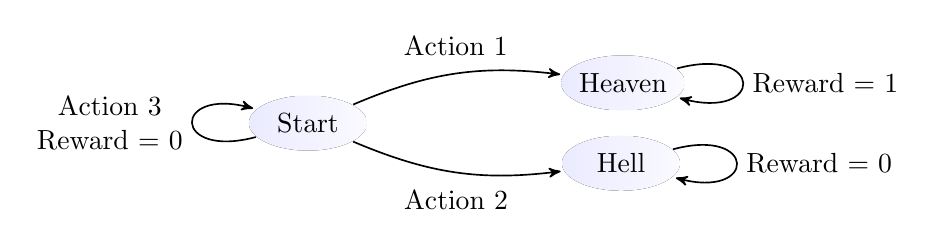
\begin{tikzpicture}[>=stealth', shorten >=1pt, auto, node distance=2.9cm, semithick]
        % Styles for uniform, larger nodes
        \tikzstyle{state} = [ellipse, minimum width=1.5cm,minimum height=.7cm, inner sep=0,path picture={\fill[left color=blue!8, right color=blue!2] (path picture bounding box.south west) rectangle (path picture bounding box.north east);}]

        % States
        \node[state] (S1) {Start};
        \node[state, above right=0cm and 2.9cm of S1] (Heaven) {Heaven};
        \node[state, below right=0cm and 2.9cm of S1] (Hell) {Hell};

        % Arrows
        \path[->] (S1) edge[bend left=15] node[midway, above=.1cm] {Action 1} (Heaven)
                       edge[bend right=15] node[midway, below=.1 cm] {Action 2} (Hell);
        \path[->] (Heaven) edge[loop right] node[right] {Reward = 1} (Heaven);
        \path[->] (S1) edge[loop left] node[left, align=center] {Action 3\\ Reward = 0} (S1);        
        \path[->] (Hell) edge[loop right] node[right] {Reward = 0} (Hell);

    \end{tikzpicture}
    \caption{A variant of \Cref{fig:heaven_hell_problem} which could be called the ``Heaven or Hell or Purgatory'' problem. Now a third action is available which keeps the agent in the starting state and provides reward 0. Action 3 is always safe, as it avoids Hell and retains the option to enter Heaven. However, Action 1 leads to much higher reward and is also safe. This example shows that knowing a safe policy upfront does not resolve the Heaven or Hell problem, since the agent can only obtain high reward if it reaches Heaven, and knowing that Action 3 is safe does not help the agent to determine whether Action 1 or Action 2 will lead to Heaven.}
    \label{fig:purgatory}
\end{figure}


\paragraph{A strictly safe policy is known.} Another option is to assume that a safe policy $\pi_0$ is known upfront \citep{liu2021learning,stradi2024learning}. Not only is this a strong assumption, it is also insufficient: there exist simple instances where $\pi_0$ produces low reward, but the agent has no safe way to explore beyond $\pi_0$ (\Cref{fig:purgatory}). In order to allow the agent to safely explore beyond $\pi_0$, the two references above both also assume a multi-episode setting and assume that $\pi_0$ is ``strictly safe'', i.e., it satisfies the safety constraints with slack.


\subsection{Allowing external help.}

We avoid repeating information from \Cref{sec:related}, so we have just two points we wish to add here. First, we mentioned that \citet{kosoy_delegative_2019} relies on Bayesian inference, but it is worth noting that the majority of papers in this category rely on Bayesian inference \citep{cohen_pessimism_2020, cohen_curiosity_2021, mindermann_active_2018}. These papers also face Bayesian inference's tractability challenges, as discussed in \Cref{sec:related}. To our knowledge, the only prior papers which use external help to obtain safety guarantees without Bayesian inference are \citep{maillard_active_2019,plaut_avoiding_2024}.

Second, several papers which we list under ``focus is safety only'' do include guarantees relating to the agent's reward \citep{cohen_pessimism_2020, cohen_curiosity_2021}. However, those guarantees are of the form ``define regret relative to prior errors'' and thus are subject to the weaknesses discussed previously.

\subsection{Other related work} 

The idea of designing agents which act cautiously when uncertain is not novel. Indeed, this idea is so fundamental that the prior work on this topic far outstrips what we can cover here. Representative theoretical papers include \citet{cortes2018online, hadfield-menell_inverse_2017, li2008knows}. Our model is also reminiscent of active learning \citep{hanneke2014active} due to how the agent proactively requests information and of imitation learning \citep{osa_algorithmic_2018} due to how the agent attempts to imitate the mentor. However, we are not aware of any relevant technical implications. Finally, see \citet{garcia_comprehensive_2015,gu_review_2024, krasowski_provably_2023} for surveys of the safe RL literature.



\section{Comprehensive discussion of \citet{plaut_avoiding_2024}}\label{sec:ac-full}

This section provides technical details relating to \citet{plaut_avoiding_2024} which were omitted from \Cref{sec:ac-overview}. We also reproduce the pseudocode for their Algorithm 1 here for convenience.

\subsection{Comprehensive comparison between our model and that of \citet{plaut_avoiding_2024}}

\Cref{tab:model-comparison-full} provides a complete list of the differences between our models. The first four were already covered in \Cref{sec:ac-overview}, but we discuss the last three here.


\paragraph{Source of next state.} In an MDP, each state is generated by the transition kernel $P$. In the online learning literature (and in \citet{plaut_avoiding_2024}), each state is generated by an adversary as a function of the events of all previous timestamps.\footnote{One can also consider a non-adaptive or ``oblivious'' adversary, but \citet{plaut_avoiding_2024} allow adaptive adversaries.} Clearly an MDP transition kernel is one way for the adversary to choose the next state, so any result which applies to all adversaries also applies to an MDP transition kernel.

\input{model_comparison_full}

\paragraph{Smoothness.} A $\sigma$-smooth adversary cannot directly pick $s_t$ but must sample $s_t$ from a distribution
$\mathcal{D}_t$ whose concentration is upper-bounded by $1/\sigma$ times the uniform distribution. In an MDP, $s_t$ is sampled from the distribution $P(s_{t-1}, a_{t-1})$, so a $\sigma$-smooth adversary corresponds to a $\sigma$-smooth $P$ as defined in \Cref{sec:model}.

\paragraph{Agent observations.} In most of the online learning literature, the agent observes each reward it obtains. However, \citet{plaut_avoiding_2024} actually do not allow the agent to observe rewards. This is because in their model, each reward represents the chance of catastrophe on the time step. In most scenarios, one only observes whether catastrophe occurred, not its probability. 

In MDPs, typically the agent does observe rewards, since this is the only way for it to learn which states and actions are good. However, observing rewards turns out to be irrelevant for our results. This is because (1) our reduction does not utilize any reward observations and (2) the algorithm from \citet{plaut_avoiding_2024} is assumed to not observe rewards, as mentioned.


\section{The general case: Proof of \texorpdfstring{\Cref{thm:main-decomp}}{Theorem 1.6}}\label{sec:algo}

First, we show that data structure of \Cref{l:max_min_query} can be used to compute distances witnessed by shortest paths that pass through a constant-size separator.

\begin{lemma}\label{l:single_adhesion}
Fix a constant $k \in \mathbb{N}$. There exists an algorithm which as the input receives an edge-weighted graph $G$ on $n$ vertices and $m$ edges together with a partition of its vertices into three sets $A, B, C$ such that $|B| \leq k$ and there are no edges between $A$ and $C$, and as the output computes $\max_{c \in C} \dist(a, c)$ for every $a \in A$. The running time is $\Oh(m \log n + n \log^{k - 1} n)$.
\end{lemma}

\begin{proof}
Let $B = \{b_1, \ldots, b_k\}$. For any $a \in A, c \in C$, we have $\dist(a, c) = \min_{i \in [k]} \dist(a, b_i) + \dist(c, b_i)$. First, we run Dijkstra's algorithm from every vertex in $B$ to find $\dist(v, b_i)$ for every $v \in V(G)$ and $i \in [k]$. Next, we use \Cref{l:max_min_query} to construct a data structure $\mathbb{D}$ for the point set $\{(\dist(c, b_1), \dots, \dist(c, b_k))\colon c\in C\}\subseteq \mathbb{R}^k$. Now, the value $\max_{c \in C} \dist(a, c)$ for any given $a$ is equal to the answer of $\mathbb{D}$ to the query with argument $(\dist(a, b_1), \dots, \dist(a, b_k))$.
\end{proof}

After computing the distances over a constant-size separator, we will use the following observation to simplify one of the sides of the separation.

\begin{lemma}\label{l:inserting_paths}
Let $G$ be a edge-weighted connected graph and let $A, B, C$ be a partition of its vertices such that there are no edges between $A$ and $C$. For every pair of vertices $u, v \in B$, let $P_{u, v}$ be any shortest path from $u$ to $v$ with all internal vertices in $C$ (assuming such a path exists).

Let $G'$ denote a graph obtained from $G[A \cup B]$ by adding an edge from $u$ to $v$ of weight equal to the length of $P_{u, v}$, for all $u, v \in B$ for which $P_{u, v}$ exists. Then,  $$\dist_G(s, t) = \dist_{G'}(s, t)\qquad\textrm{for all }s,t\in A\cup B.$$
\end{lemma}
\begin{proof}
Let $G''$ be the graph obtained by adding new edges of $G'$ to $G$.
Fix any $s, t \in A \cup B$ and let $P$ denote the shortest path from $s$ to $t$ in $G''$ which minimizes the number of vertices from $C$ visited. Naturally, the weight of $P$ is equal $\dist_G(s, t)$. Assume that such path visits at least one vertex of $C$. Then, the path $P$ is of the form $s \xrightarrow{P_1} x \xrightarrow{P_2} y \xrightarrow{P_3} t$, where $x, y \in B$ and all the internal vertices of $P_2$ are in $C$. By the construction of $G'$, $P_2$ can be replaced with a direct edge from $x$ to $y$ of the same weight. We obtain a same weight path with a smaller number of vertices of $C$ visited, which is a contradiction. Therefore, $P$ is entirely contained in $A \cup B$, hence it exists in $G'$. This shows that $\dist_G(s, t) = \dist_{G'}(s, t)$.
\end{proof}


The next lemma encapsulates the main algorithmic content of the proof of \Cref{thm:main-decomp}. The algorithm will split the tree decomposition provided on input into smaller parts for which the eccentricities are easier to calculate. We use the following lemma to handle a single such part.
\begin{lemma}\label{l:star}
Fix constants $k, g \in \mathbb{N}, 0 < \delta < \frac{1}{54}$. Assume we are given $n \in \mathbb{N}$, an edge-weighted graph $G$ on at most $n$ vertices with a weight function $w \colon E(G) \to \mathbb{N}$, a vertex subset $A$ and a collection of non-empty vertex subsets $V_0, V_1, \dots, V_\ell$ satisfying the following conditions:
\begin{itemize}[nosep]
	\item The sum of weights of all the edges in $G$ is bounded by $\Oh(n)$.
	\item $V(G) \setminus A = V_0 \cup V_1 \cup \dots \cup V_\ell$.
	\item $|A| \leq k$.
	\item For every $i \in [\ell]$, $G[V_i \setminus V_0]$ is connected, $N_G(V_i \setminus V_0) = V_i \cap V_0$, $|V_i| = \Oh(n^\delta)$, and $|V_0 \cap V_i| \leq 4$.
	\item For all $i, j \in [\ell], i \neq j$, $V_i \setminus V_0$ and $V_j \setminus V_0$ are disjoint and non-adjacent in $G$.
	\item Every edge $uv \in E(G)$ with $u, v \not\in A$ is contained in $G[V_i]$ for some $i\in \{0,1,\ldots,\ell\}$.
	\item The graph obtained by taking $G[V_0]$ and adding a clique on $V_0 \cap V_i$ for every $i \in [\ell]$ has Euler genus bounded by $g$.
\end{itemize}
Then, we can compute the eccentricity of every vertex of $G$ in time $\Oh \left( n^{1 + \frac{150 + 54 \delta}{151}} \log^k n \right)$.
\end{lemma}

\begin{proof}
Fix $\delta' = \frac{1 + 97 \delta}{151}$; we have $\delta' - \delta = \frac{1 - 54\delta}{151} > 0$.
Let $E_i$ denote the set of edges with one endpoint in $V_i$ and the other endpoint in $V_i \setminus V_0$. For $i \in [\ell]$, we shall say that $V_i$ is {\em{heavy}} if the sum of weights of $E_i$ is larger than $n^{\delta'}$. Since the sets $E_i$ are pairwise disjoint and the total sum of weights of all the edges is bounded by $\Oh(n)$, the number of heavy subsets is bounded by $\Oh(n^{1 - \delta'})$. Without loss of generality, we may assume that $V_{\ell' + 1}, \dots, V_\ell$ are heavy and $V_1, \dots, V_{\ell'}$ are not, for some $\ell'\in \{0,\ldots,\ell\}$.


For any source vertex $s$, we can calculate distances from $s$ to every vertex of $G$  using breadth first search in time $\Oh(\sum_{e \in E(G)} w(e)) = \Oh(n)$.
In particular, for every $\ell' < i \leq \ell$, we can compute the distances from every vertex of $V_i$ to every vertex of $G$ in total time $\Oh(n^{2 - \delta' + \delta})$, because $$|V_{\ell'+1}\cup \ldots\cup V_{\ell}|\leq n^{1-\delta'}\cdot \Oh(n^\delta)=\Oh(n^{1-\delta'+
\delta}).$$
Additionally, we calculate distances $\dist_G(a, v)$ for every $a \in A, v \in V(G)$ in time $O(n)$.

For every $i \in [\ell]$ and $u,v \in V_0 \cap V_i$, there exists a shortest path $P_{i,u,v}$ from $u$ to $v$ with all internal vertices belonging to $V_i - V_0$ due to the assumption that $G[V_i - V_0]$ is connected and $N_G(V_i - V_0) = V_i \cap V_0$. Therefore, the distance from $u$ to $v$ is bounded by the sum of weights of edges in $E_i$. In particular, for $i \in [\ell']$, $\dist_G(u, v) \leq n^{\delta'}$.

We define $\widetilde{G}$ to be the graph obtained by taking $G[A \cup V_0 \cup \dots \cup V_{\ell'}]$ and applying the following operation for every $i \in \{\ell' + 1, \dots, \ell\}$:
for each pair of vertices $u, v \in A \cup (V_0 \cap V_i)$, add an edge in $\widetilde{G}$ between $u$ and $v$ with weight equal to the total weight of $P_{i,u,v}$. For a fixed $i, u$, we can find $P_{i, u, v}$ for all $v$ using breadth first search in time $\Oh(n)$. Taking a sum over all $i, u$, we get that $\tilde{G}$ can be computed in total time $\Oh(n^{2 - \delta'})$.


\begin{claim}\label{cl:wG}
The sum of the edge weights in $\widetilde{G}$ is $\Oh(n)$. Moreover, for all $u, v \in V(\widetilde{G})$, we have $\dist_{\widetilde{G}}(u, v) = \dist_{G}(u, v)$.
\end{claim}

\begin{proof}
Consider $i \in \{\ell' + 1, \dots, \ell\}$ and any $u, v \in A \cup (V_0 \cap V_i)$ for which we added an edge. Its weight is bounded by the sum of weights of edges in $E_i$. Therefore, the total weight of all edges added is at most
$$
\sum_{i \in \{\ell' + 1, \dots, \ell\}} \left( |A \cup (V_0 \cap V_i)|^2 \sum_{e \in E_i} w(e) \right) \leq (4 + k)^2 \sum_{e \in E(G)} w(e) = \Oh(n).
$$
This proves the first part of the claim.

For the second part of the claim, consider any $i \in \{\ell' + 1, \dots, \ell \}$ and observe that by our assumptions, $A \cup (V_0 \cap V_i)$ separates $(V_0 \cup \dots \cup V_{\ell'} \cup V_{i + 1} \cup \dots \cup V_\ell) \setminus V_i$ from $V_i \setminus V_0$. Hence it suffices to repeatedly apply \Cref{l:inserting_paths}.
\end{proof}

For every $u \in V(\widetilde{G})$, we have $\ecc_G(u) = \max(\ecc_{\widetilde{G}}(v), \max_{v \in V(G) \setminus V(\widetilde{G})} \dist_G(u, v))$. Note, that we already know all the distances $\dist_G(u, v)$ for $v \in V(G) \setminus V(\widetilde{G})$. Similarly, we can already compute $\ecc_G(u)$ for every $u \in V(G) \setminus V(\widetilde{G})$. Therefore, it remains to compute $\ecc_{\widetilde{G}}(v)$ for each $v \in V(\widetilde{G})$. Our goal is to show that this can be done efficiently using \Cref{l:main_ecc}.

Now, let $G'$ be the graph obtained from $\tilde{G}$ by replacing every edge $e$ non-indicent to $A$ with $w(e)\geq 2$ with a path of length $w(e)$ consisting of unit-weight edges. This operation again preserves the distances. Since the sum of edge weights in $\tilde{G}$ is of $\Oh(n)$, the total number of vertices in $G'$ is of $\Oh(n)$. For $0 \leq i \leq \ell'$, we write $V'_i$ to denote the set $V_i$ together with all the vertices added as a part of a path between two endpoints in $V_i$.
As $V_i$ is not heavy for each $i\in [\ell']$, we have
$$
|V'_i \setminus V'_0| \leq |V_i| + \sum_{e \in E_i} w(e) = \Oh(n^{\delta'})\qquad \textrm{for all }i\in [\ell'].
$$

Let $G_0$ denote the graph $G'[V'_0]$ and let $G_0^*$ denote the graph $G'- A$ with $V'_i - V'_0$ contracted to a single vertex $v_i^*$, for each $i \in [\ell']$; note that, all edges of $G_0$ and $G_0^*$ have unit weight.

\begin{claim}
	The graph $G_0^*$ is does not contain $K_{t}$ as a minor, where $t = \Oh(\sqrt{g})$.
\end{claim}

\begin{proof}
Let $\bar{G}_0$ denote the graph obtained by taking $G_0$ and adding a clique on $V_0 \cap V_i$ for every $i \in [\ell']$.
By lemma assumptions and the fact that subdividing edges does not increase the Euler genus, $\bar{G}_0$ has Euler genus at most $g$. In particular, $\bar{G}_0$ is $K_{t'}$-minor-free for some $t' = \Oh(\sqrt{g})$, because the Euler genus of $K_{t'}$ is $\Omega({t'}^2)$.

Similarly, let $\bar{G}_0^*$ be the graph obtained by taking $G_0^*$ and adding a clique on each $V_0 \cap V_i$.
Note, that $\bar{G}_0^* - \{v_1^*, \dots, v_{\ell'}^*\}$ is precisely $\bar{G}_0$. Let $t = \max(t', 6)$.
Recall that a minor model of a clique $K_t$ consists of $t$ pairwise vertex-disjoint connected subgraphs, called
branch sets, such that there is at least one edge between each pair of the branch sets.
Consider a minor model $\varphi$ of $K_{t}$ in $\bar{G}^*_0$.
Note that $\varphi$ cannot contain any singleton branch set of the form $\{v^*_i\}$, for the degree of $v^*_i$ in $\bar{G}^*_0$ is at most $4 < t - 1$. Furthermore, since $N_{\bar{G}^*_0}(v^*_i) = V_0 \cap V_i$, any branch set containing $v^*_i$ and at least one other vertex contains some $u \in V_0 \cap V_i$, and $N_{\bar{G}^*_0}(v^*_i)\subseteq N_{\bar{G}^*_0}(u)$, hence removing $v^*_i$ from this branch set preserves the model. Therefore, we can assume without loss of generality that all branch sets of $\varphi$ are disjoint from $\{v^*_1, \dots, v^*_{\ell'}\}$, hence $\varphi$ is a minor model of $K_{t}$ in $\bar{G}_0$. This is a contradiction, as $t \geq t'$ and $\bar{G}_0$ is $K_{t'}$-minor-free. Therefore, $\bar{G}_0^*$ is $K_t$-minor-free, hence $G_0^*$ also.
\end{proof}

Let $\rho' = \frac{2 - 108 \delta}{151} > 0$. The graph $G^*_0$ is a unit-weight graph and is $K_{t}$-minor-free.
Hence, by applying \Cref{t:r_division} to $G^*_0$ (with $\varepsilon = \rho'/2$)
we obtain an $n^{\rho'}$-division $\mathcal{R}_0$ in time $\Oh(n^{1 + \rho'})$.
We extend it to $G' - A$ by mapping every contracted vertex $v^*_i$ to $N_{G' - A}[V'_i - V'_0] = (V'_i - V'_0) \cup (V_0 \cap V_i)$. Formally, we put $V''_i \coloneqq N_{G' - A}[V'_i - V'_0]$ and 
$$
\mathcal{R} \coloneqq \left\{ (R_0 \cap V'_0) \cup \bigcup_{i \colon v^*_i \in R_0} V''_i \colon R_0 \in \mathcal{R}_0 \right\}.
$$

Now, we argue that $\mathcal{R}$ is a reasonable division of $G' - A$. Clearly, all sets $R \in \mathcal{R}$ are connected in $G' - A$. Pick any $R \in \mathcal{R}$ and let $R_0$ be its corresponding set in $\mathcal{R}_0$.
Every vertex $v^*_i$ is mapped to a set of size $\Oh(n^{\delta'})$, therefore
$$|R| \leq |R_0| \cdot \Oh(n^{\delta'}) = \Oh(n^{\rho' + \delta'}).$$

By our construction, for every $i \in [\ell']$, $R$ is either disjoint from $V'_i - V'_0$ or contains whole $N_{G' - A}[V'_i - V'_0]$. This means that no vertex belonging to any $V'_i - V'_0$ can be in $\partial R$, hence $\partial R \subseteq V'_0$.

Pick any $u \in \partial R \cap R_0$. Assume that $u \not\in \partial R_0$. Then every vertex of $N_{G_0^*}(u)$ must be in $R_0$, hence $N_{G - A'}(u) \subseteq R$, which is a contradiction. This means that $\partial R \cap R_0 \subseteq \partial R_0$.

Pick any $u \in \partial R - R_0$. Then, $u \in V_0 \cap V_i$ for some $i \in [\ell']$ such that $v_i^* \in R_0$. Moreover, $v_i^* \in \partial R_0$ and is adjacent to $u$ in $G_0^*$. The number of such $u$ is bounded by $4 |\partial R_0 \cap \{ v_1^*, \dots, v_{\ell'}^* \}|$.

Putting two cases together, we obtain:
$$
\sum_{R \in \mathcal{R}} |\partial R| = \sum_{R \in \mathcal{R}} \left(|\partial R \cap R_0| + |\partial R - R_0|\right) \leq \sum_{R_0 \in \mathcal{R}_0} \left(|\partial R_0| + 4 |\partial R_0 \cap \{ v_1^*, \dots, v_{\ell'}^* \}|\right) = \Oh(n^{1 - \frac{1}{2}\rho'}).
$$

It remains to show the following claim.

\begin{claim}
Pick any $R \in \mathcal{R}, s_R \in R$. The number of different distance profiles on $R$ relative to $s_R$ in $G' - A$ is of $\Oh(n^{48\rho' + 54\delta'})$.
\end{claim}
\begin{proof}
We look at every vertex $v \in V(G') \setminus A$ and consider three cases: $v \in R$, $v \in V'_0$, and $v \in V'_i \setminus (V'_0 \cup R)$ for some $i \in [\ell']$. By our construction, $R \cap V'_0$ is non-empty, hence w.l.o.g. we can assume that $s_R \in V'_0$ as whether two vertices have the same profile on $R$ is independent of the choice of the pivot vertex.

In the first case, there are at most $|R| = \Oh(n^{\rho' + \delta'})$ such vertices, hence they realise at most that many profiles.

In the second case, we want to observe that profile of any vertex $v \in V'_0$ on $R$ depends only on its profile on $R \cap V'_0$ (relative to $s_R$). Pick any $t \in R - V'_0$. Then $t \in V'_i - V'_0$ for some $i \in [\ell']$, $V_i \cap V_0 \subseteq R \cap V'_0$, and every path from $v$ to $t$ intersects $V_i \cap V_0$. In particular, distances from $v$ to vertices of $V_i \cap V_0$ determine its distance to $t$, which proves the observation.

Let $\tilde{G}_0$ denote the graph obtained by taking $G'[V'_0]$ and for every $i \in [\ell'], u, v \in V_0 \cap V_i$ adding a disjoint path from $u$ to $v$ of length $\dist(u, v)$. Let $P_i$ denote the vertex set of paths added between $V_0 \cap V_i$. For every $t \in V'_0$ we have $\dist_{G' - A}(v, t) = \dist_{\tilde{G}_0}(v, t)$, so it suffices to bound the number of profiles on $R \cap V'_0$ in $\tilde{G}_0$. By our assumptions, $\tilde{G}_0$ has Euler genus bounded by $g$ and all $P_i$ are of size $\Oh(n^{\delta'})$.

Let $R_0$ be the set of $\mathcal{R}_0$ corresponding to $R$. Let $\tilde{R}_0$ denote the set $(R \cap V'_0) \cup \bigcup_{i : v^*_i \in R_0} P_i$. Such set is connected in $\tilde{G}_0$. Moreover, similarly to $R$, its size is $\Oh(n^{\rho' + \delta'})$. Applying \Cref{thm:distprofiles}, we get that the number of distance profiles on $\tilde{R}_0$ in $\tilde{G}_0$ is $\Oh(n^{12(\rho' + \delta')})$, which also bounds the number of profiles on $R$ in $G' - A$ realised by $V'_0$.

For the third case, assume $v \in V'_i \setminus (V'_0 \cup R)$ for some $i\in [\ell']$. Every path from $v$ to any vertex of $R$ in $G' - A$ intersects $V_i \cap V_0$. Let $v_1, \dots v_p$ be the vertices of $V_i \cap V_0$, where $p \leq 4$. The profile of $v$ on $R$ is then determined by the following:
\begin{itemize}[nosep]
 \item[(a)] the profile of each $v_j$ on $R$,
 \item[(b)] $\dist_{G' - A}(v, v_j) - \dist_{G' - A}(v, v_1)$ for each $2 \leq j \leq p$, and
 \item[(c)] $\dist_{G' - A}(s_R, v_j) - \dist_{G' - A}(s_R, v_1)$ for each $2 \leq j \leq p$ where $s_R$ is some pivot vertex of $R$.
\end{itemize}
By the previous case, the number of distance profiles of each $v_j$ is $\Oh(n^{12(\rho' + \delta')})$. The distances between $v$ and $v_j$ are bounded by $|V'_i|$, hence each quantity described in (b) can take $\Oh(n^{\delta'})$ different possible values. Similarly, since $v_1$ and $v_j$ are connected via $V'_i$, $|\dist_{G' - A}(s_R, v_j) - \dist_{G' - A}(s_R, v_1)| \leq \Oh(n^{\delta'})$. The number of different possible profiles of such $v$ is therefore bounded by $\Oh(n^{48(\rho' + \delta') + 6\delta'}) = \Oh(n^{48\rho' + 54\delta'})$. This finishes the proof of the claim.
\end{proof}

Now we can apply \Cref{l:main_ecc} to graph $G'$ with apex set $A$, $X = V(\widetilde{G})$, and the following constants: $$\rho = \rho' + \delta',\qquad \gamma = 1 - \frac{1}{2}\rho',\quad \textrm{and}\quad \alpha = 48\rho' + 54 \delta'.$$ This allows us to calculate all $V(\widetilde{G})$-eccentricities in $G'$ in time
$$
\Oh \left( \left(
	n^{ 2 - \frac{1}{2} \rho' } +
	n^{ 1 + 48\rho' + 54 \delta' }
\right) \log^k n \right) =
\Oh \left( n^{1 + \frac{150 + 54 \delta}{151}} \log^k n \right).
$$
Since for each $v\in V(\widetilde{G})$ we have $\ecc_{\widetilde{G}}(v) = \max_{u \in V(\widetilde{G})} \dist_{\widetilde{G}}(v, u) = \max_{u \in V(\widetilde{G})} \dist_{G'}(v, u)$, this means that we have successfully computed all the eccentricities in $\widetilde{G}$; and as we argued, this is enough to compute all the eccentricities in $G$ as well.

Finally, the total running time of the algorithm is
$$
\Oh \left( n^{1 + \frac{150 + 54 \delta}{151}} \log^k n + n^{2 - \delta' + \delta} \right) =
\Oh \left( n^{1 + \frac{150 + 54 \delta}{151}} \log^k n \right).
$$\qedhere
\end{proof}


\begin{lemma}\label{l:star2}
Fix constants $k, g \in \mathbb{N}, 0 < \delta < \frac{1}{54}$. Assume we are given $n \in \mathbb{N}$, an edge-weighted graph $G$ on at most $n$ vertices with a weight function $w \colon E(G) \to \mathbb{N}$, a vertex subset $A$ and a collection of non-empty vertex subsets $V_0, V_1, \dots, V_\ell$ satisfying the same conditions as in \Cref{l:star} with the following differences:
\begin{itemize}
	\item we don't require $G[V_i - V_0]$ to be connected and $V_i - V_0$ to be adjacent to whole $V_i \cap V_0$;
	\item instead of $|V_0 \cap V_i| \leq 4$, we require $|V_0 \cap V_i| \leq k$.
\end{itemize}
Then, we can compute the eccentricity of every vertex of $G$ in time $\Oh \left( n^{1 + \frac{150 + 54 \delta}{151}} \log^{k + 5g} n \right)$.
\end{lemma}

\begin{proof}
We will reduce our input to one which will satisfy the conditions of \Cref{l:star}. We start by addressing the adhesions $V_0 \cap V_i$ containing too many vertices.

Let $G_0$ denote the graph $G[V_0]$ with cliques placed at $V_0 \cap V_i$ for every $i \in [\ell]$.
For every $i \in [\ell]$ we repeat the following procedure: while $|V_0 \cap V_i| > 4$,
remove arbitrary $5$ vertices from $V_0 \cap V_i$. Since $|V_0 \cap V_i| \leq k$ for each $i\in [\ell]$,
this procedure can be implemented in total time $\Oh(n)$. As a result, at the end we have $|V_0 \cap V_i| \leq 4$ for all $i \in [\ell]$. Let $M$ be the set of all the removed vertices. By our assumptions, $G_0$ has Euler genus bounded by $g$, hence it cannot contain $g + 1$ pairwise disjoint copies of $K_5$
(as the Euler genus of a graph is the sum of the Euler genera of its 2-connected components~\cite{StahlB77} and $K_5$ is not planar). Each removed quintiple of vertices induces a $K_5$ in $G_0$, hence we have $|M| \leq 5g$. We set $A' = A \cup M$ and may thus assume that $V_i$ is disjoint from $A'$ for all $0 \leq i \leq \ell$.

Now, fix $i \in [\ell]$. Let $C^i_1, \dots, C^i_{r_i}$ denote the connected components of $V_i - V_0$ in $G - A'$. We define $W^i_j := N_{G - A'}[C^i_j]$ for every $j \in [r_i]$. Clearly, all $W^i_j$ induce a connected subgraph of $G$ and satisfy $N_{G - A'}(W^i_j - V_0) = W^i_j \cap V_0$. We put $V'_0 := V_0$ and enumerate
$$
\{V'_1, V'_2, \dots V'_{\ell'}\} := \{ W^i_j \colon i \in [\ell], j \in [r_i] \}.
$$
It is easy to verify that the sets $A'$ and $V'_0, V'_1, \dots, V'_{\ell'}$ satisfy the conditions of \Cref{l:star}. We apply said lemma to calculate the eccentricity of every vertex of $G$ in the desired time.
\end{proof}



The next statement is a reformulation of \Cref{thm:main-decomp}.

\begin{theorem}
Fix constants $k, g \in \mathbb{N}$. Assume we are given a graph $G$ on $n$ vertices together with its tree decomposition $(T, \beta)$ and a set of private apices $A_t \subseteq \beta(t)$ for each node $t\in V(T)$ such that the following conditions hold:
\begin{itemize}[nosep]
 \item For every node $t \in V(T)$, we have $|A_t| \leq k$.
 \item For every edge $st \in E(T)$,  we have $|\beta(v) \cap \beta(u)|\leq k$.
 \item For every node $t \in V(T)$, graph obtained by taking $G[\beta(t)] - A_t$ and turning  $(\beta(t) \cap \beta(s))\setminus A_t$ into a clique for every edge $st \in E(T)$ has Euler genus bounded by $g$.
\end{itemize}
Then, we can compute the eccentricity of every vertex of $G$ in time $\Oh \left( n^{1 + \frac{355}{356}} \log^{k + 5g} n \right)$.
\end{theorem}

\begin{proof}
We may assume that $|V(T)|\leq n$, for every tree decomposition with no two bags comparable by inclusion has this property; and adjacent comparable bags can be merged by contracting the edge between them.

For a node $t\in V(T)$, by the {\em{weight}} of $t$ we mean the size of the corresponding bag, that is, $|\beta(t)|$. For any subset of nodes $S \subseteq V(T)$, we define $\beta(S) \coloneqq \bigcup_{t \in S} \beta(t)$ By the {\em{weight}} of $S$, we mean the total weight of the elements of $S$, that is, $\sum_{t\in S} |\beta(t)|$. 

\begin{claim}\label{cl:weight-T}
The weight of $V(T)$ is of $\Oh(n)$.
\end{claim}

\begin{proof}
The sets $\beta'(t) := \beta(t) - \bigcup_{s \in N_T(t)} \beta(s)$ are pairwise disjoint. We have
$$
\sum_{t \in V(T)} |\beta(t)| =
\sum_{t \in V(T)} |\beta'(t)| + 2 \cdot \sum_{st \in E(T)} |\beta(s) \cap \beta(t)| \leq
|V(T)| + 2k|E(T)| = \Oh(n).
$$
\end{proof}

Since every bag induces a graph of bounded Euler genus, the number of edges contained in a bag is linear in its size. In particular, this implies that the total number of edges of $G$ is also bounded by $\Oh(n)$.

We set $$\delta \coloneqq \frac{1}{356}\qquad\textrm{and}\qquad \Delta \coloneqq \frac{355}{356}.$$ Root the tree $T$ in an arbitrarily chosen node; this naturally imposes an ancestor-descendant relation in $T$ (for convenience, every node is considered its own ancestor and descendant).

We start by partitioning $T$ into connected subtrees using the following procedure.
We proceed bottom-up over $T$, processing nodes in any order so that a node is processed after all its strict descendants have been processed. Along the way, we mark some nodes and split the edges of $T$ into heavy and light. Let $t \in V(T)$ be the currently processed non-root node of $T$ and let $e \in E(T)$ be the edge connecting $t$ with its parent. If the total weight of all the unmarked nodes that are descendants of $t$ is at least $n^\delta$ (recall that this includes $t$ itself as well), then we declare $e$ heavy and mark all the descendants of $t$ that were unmarked so far. Otherwise, the edge $e$ is declared light and the procedure proceeds to further nodes of $T$.

Observe that
removing all heavy edges splits $T$ into connected subtrees, say $T'_1, \cdots T'_m$. All of the subtrees, except for possibly the subtree containing the root node, are of weight at least $n^\delta$. In particular, the number of subtrees $m$, and therefore the number of heavy edges, is  bounded by $\Oh(n^{1 - \delta})$. Moreover, in every subtree $T'_i$, removing the node closest to the root splits $T'_i$ into smaller components, each of weight less than $n^\delta$.

Fix a heavy edge $e$ and let $T^e_1$ and $T^e_2$ be the two subtrees into which $T$ splits after removing~$e$. Let $X^e_i = \beta(T^e_i)$ for $i \in \{1, 2\}$. Put $A_e = X^e_1 \setminus X^e_2$, $C_e = X^e_2 \setminus X^e_1$, and $B_e = X^e_1 \cap X^e_2$. By the properties of tree decompositions, such choice of $A_e, B_e, C_e$ satisfies the conditions of \Cref{l:single_adhesion}, hence in time $\Oh(n \log^{k - 1} n)$ we can compute $\max_{v \in X^e_2} \dist_G(u,v)$ for every $u \in X^e_1$, and $\max_{u \in X^e_1} \dist_G(u,v)$ for every $v \in X^e_2$. Computing this for every heavy edge $e$ takes total time $\Oh(n^{2 - \delta} \log^{k - 1} n)$.

Fix any subtree $T'=T'_j$. Let $e_1 = t^{e_1}_1t^{e_1}_2, e_2 = t^{e_2}_1 t^{e_2}_2, \dots, e_\ell = t^{e_\ell}_1 t^{e_\ell}_2$ denote the heavy edges incident to $T'$, where $t^{e_i}_1 \in V(T')$ and $V(T') \subseteq V(T_1^{e_i})$ for every $i \in [\ell]$.
For a vertex $v \in \beta(T')$, let
$$d_0(v) = \max_{u \in \beta(T')} \dist_G(v, u)\qquad\textrm{and}\qquad d_i(v) = \max_{u \in X_2^{e_i}}\dist_G(v,u),\quad\textrm{for } i \in [\ell].$$ We have $\ecc(v) = \max \{ d_i(v)\colon i\in \{0,1,\ldots,\ell\}\}$.The values of $d_i(v)$ are already calculated for all $i\in [\ell]$, hence it remains to compute $d_0(v)$.

For every $i \in [\ell]$ and every pair of vertices $u, v \in \beta(t^{e_i}_1) \cap \beta(t^{e_i}_2)$ we find a shortest path between $u$ and $v$ with all internal vertices inside $X^{e_i}_2$ (or determine that it doesn't exist). For a fixed $u, v$ this can be done in time $\Oh(n)$. Since in total we perform this step at most $2k^2$ times per heavy edge, it takes $\Oh(n^{2 - \delta})$ time in total. Let $P_{i, u, v}$ denote such path, assuming it exists.

Let $G'$ denote the graph obtained from $G[\beta(T')]$ by taking every $i, u, v$ for which $P_{i, u, v}$ exists and adding an edge between $u$ and $v$ of weight equal to the total weight of $P_{i, u, v}$.
The weight of every edge inserted in $\beta(t^{e_i}_1) \cap \beta(t^{e_i}_2)$ is bounded by $|X^{e_i}_2|+1$. The total weight of all edges inserted is therefore at most
$$
\sum_{i \in [\ell]} |\beta(t^{e_i}_1) \cap \beta(t^{e_i}_2)|^2 \cdot (|X^{e_i}_2|+1) \leq
k^2 \sum_{i \in [\ell]} (|X^{e_i}_2|+1) = \Oh(n),
$$
where the last equality follows from the fact that all the trees $T^{e_i}_2$ are pairwise disjoint.
By \Cref{l:inserting_paths}, we have $\dist_{G'}(u, v) = \dist_G(u, v)$ for each $u, v \in \beta(T')$. Hence, computing $d_0(v)$ for every $v \in \beta(T')$ is equivalent to computing the eccentricity of every vertex in $G'$.

If the size of $\beta(T')$ is smaller than $n^\Delta$, we compute the eccentricities naively in time $\Oh(|\beta(T')|^2)$, 
noting that $G'$ has $\Oh(|\beta(T')|)$ edges (thanks to Claim~\ref{cl:weight-T} and bounded genus assumption 
of the last bullet of the theorem statement). Otherwise, we argue that we can use the algorithm in \Cref{l:star} as follows.

Let $t$ be the node of $T'$ closest to the root. Let $s_1, \dots, s_p$ be the children of $t$ in $T$ and let $T''_i$ denote the connected component of $T' - \{t\}$ containing $s_i$. Set $V_0 = \beta(t)$ and $V_i = \beta(T''_i)$ for $i \in [p]$.

It is now easy to verify that $G'$ and sets $A, \{V_i\colon 0\leq i\leq p\}$ selected this way satisfy the assumptions of \Cref{l:star2}. This allows us to use it to compute the eccentricities in $G'$ in time
$$
\Oh \left( n^{1 + \frac{150 + 54\delta}{151}} \log^{k + 5g} n \right) =
\Oh \left( n^{1 + \frac{354}{356}} \log^{k + 5g} n \right).
$$
As we argued, from these eccentricities, we may easily compute all the eccentricities in $G$.

Now, let us analyse the total running time of the whole algorithm. We invoke \Cref{l:star} $\Oh(n^{1 - \Delta})$ times, since we apply it only to subtrees $T'_i$ of size at least $n^\Delta$. The total running time of those applications is hence
$$
\Oh \left( n^{2 + \frac{354}{356} - \Delta} \log^{k + 5g} n \right) =
\Oh \left( n^{1 + \frac{355}{356}} \log^{k + 5g} n \right).
$$
We compute the eccentricities naively for subtrees smaller than $n^\Delta$, hence the total running time of this computation is
$$
\sum_{i \in [m] \colon |\beta(T'_i)| \leq n^\Delta} |\beta(T'_i)|^2 \leq
n^\Delta \cdot \sum_{i \in m} |\beta(T'_i)| = \Oh(n^{1 + \Delta})=\Oh\left(n^{1+\frac{355}{356}}\right).
$$
The rest of computation can be done in $\Oh(n^{2 - \delta} \log^k n)$. Therefore, the whole algorithm runs in time $\Oh \left( n^{1 + \frac{355}{356}} \log^{k + 5g} n \right)$.
\end{proof}


\subsection{Another algorithm from \citet{plaut_avoiding_2024}}

In the main body, we focused on the primary algorithm from \citet{plaut_avoiding_2024} (\Cref{alg:nd}). However, they provide a second algorithm with the same guarantee of subconstant regret under different assumptions.

\begin{lemma}[Theorem D.3 in \citet{plaut_avoiding_2024}]
\label{lem:bucket-regret}
Assume that $\s \subseteq \bbr$ and that $\pi^m(s)$ switches at most $K$ times as $s$ moves from $-\infty$ to $+\infty$. Then for any $c \in (1/2,1)$ Algorithm 4 in \citet{plaut_avoiding_2024} satisfies \Cref{def:ac} with
\begin{align*}
Q_T  \le&\ (\diam(\smols)+4)T^c\\
\rac \le&\  2LKT^{1-2c}
\end{align*}
\end{lemma}

Combining \Cref{lem:bucket-regret} with \Cref{thm:main} produces the following alternative no-regret guarantee:

\begin{theorem}
\label{thm:bucket}
For any $c \in (0,1)$, Algorithm 4 from \citet{plaut_avoiding_2024} satisfies
\begin{align*}
Q_T \le&\ KLT^{2(1-c)}\\
R_T  \le&\ (1+\diam(\smols))T^c
\end{align*}
\end{theorem}

\subsection{Additive vs multiplicative subconstant regret}

See \Cref{sec:ac-overview} for the preliminary discussion of additive vs multiplicative subconstant regret. Here we formalize a connection between these two metrics. Specifically, \Cref{prop:sum-prod} states that when we take the supremum over payoff functions and payoffs are in $[0,1]$, these objectives roughly coincide. This is not an exact equivalence, but the approximation $1+x \approx \exp(x)$ for $x \approx 0$ implies that $1-\exp \big(\sum_{t=1}^T \mu_t(s_t,a_t) -\sum_{t=1}^T \mu_t^m(s_t) \big) \approx  \sum_{t=1}^T \mu_t^m(s_t) - \sum_{t=1}^T \mu_t(s_t, a_t)$ when the latter is small (e.g., the additive regret is subconstant).

\begin{restatable}{proposition}{propSumProd}
\label{prop:sum-prod}
For any MDP $\M$ and mentor policy $\pi^m$, every algorithm satisfies
\begin{align*}
0 \le&\ \sup_{\bfmu}\ \E\left[1-\exp \left(\sum_{t=1}^T \mu_t(s_t,a_t) -\sum_{t=1}^T \mu_t^m(s_t) \right)\right]\\ \le&\ \sup_{\bfmu}\  \E\left[\prod_{t=1}^T \mu_t^m(s_t) - \prod_{t=1}^T \mu_t(s_t, a_t)\right]\\
\le&\ \sup_{\bfmu}\ \E \left[\sum_{t=1}^T \mu_t^m(s_t) - \sum_{t=1}^T \mu_t(s_t, a_t)\right]
\end{align*}
\end{restatable}


We will need the following lemma for the proof:


\begin{lemma}[Lemma B.3 in \citet{plaut_avoiding_2024}]
\label{lem:pos-prod-bound}
Assume $x_1,\dots,x_T, y_1,\dots,y_T \in [0,1]$ and $x_t \ge y_t$ for all $t \in [T]$. Then
\[
\prod_{t=1}^T x_t - \prod_{t=1}^T y_t \le \sum_{t=1}^T x_t - \sum_{t=1}^T y_t
\]
\end{lemma}


\begin{proof}[Proof of \Cref{prop:sum-prod}]
Let $\U$ be the set of payoff functions satisfying $L$-local generalization; then $\mu_t \in \U$ for all $t \in [T]$ and the suprema range over $\bfmu \in \U^T$.

\textbf{Part 1: the first inequality.} Let $\nu_t(s,a) = 0$ for all $s\in \s, a \in \A, t \in [T]$. We have $\nu_t \in \U$ trivially for all $t \in [T]$, so
\[
\sup_{\bfmu}\ \E\left[1-\exp \left(\sum_{t=1}^T \mu_t(s_t,a_t) -\sum_{t=1}^T \mu_t^m(s_t) \right)\right] \ge  \E\left[1-\exp \left(\sum_{t=1}^T \nu_t(s_t,a_t) -\sum_{t=1}^T \nu_t^m(s_t) \right)\right] = 1 - \exp(0) = 0
\]
\textbf{Part 2: the second inequality.} For each $\mu \in \U$, define another payoff function $f(\mu): \s \times \A \to [0,1]$ by $f(\mu)(s,a) = 1 - \mu^m(s) + \min(\mu^m(s), \mu(s,a))$. Let $f(\mu^m)(s) = f(\mu)(s,\pi^m(s))$ for brevity. Note that $\min(\mu^m(s), \mu(s,\pi^m(s))) = \mu^m(s)$ and thus $f(\mu^m)(s) = 1 $ for all $s \in \s$.

We first claim that for all $\mu \in \U$, $f(\mu) \in \U$. For any $s,s' \in \s$, either $f(\mu)(s,\pi^m(s')) = 1 - \mu^m(s) + \mu^m(s) = 1$, or $f(\mu)(s,\pi^m(s')) = 1 - \mu^m(s) + \mu(s,\pi^m(s'))$. In the former case, we have
\[
|f(\mu^m)(s) - f(\mu)(s,\pi^m(s'))| = |1-1| = 0 \le L \norm{s-s'}
\]
and in the latter case, we have
\begin{align*}
|f(\mu^m)(s) - f(\mu)(s,\pi^m(s'))| =&\ |1 - (1 - \mu^m(s) + \mu(s, \pi^m(s')))|\\
=&\ |\mu^m(s) - \mu(s,\pi^m(s'))|\\
\le&\ L\norm{s-s'}
\end{align*}
with the last step due to $\mu \in \U$. Therefore $f(\mu) \in \U$. Now fix any $s_1,\dots,s_T$ and $a_1,\dots,a_T$. Using the standard inequality $\log(1+x) \le x$ for all $x \in \bbr$,
\begin{align*}
\prod_{t=1}^T f(\mu_t)(s_t, a_t) =&\ \exp \sum_{t=1}^T \log \big(f(\mu_t)(s_t, a_t)\big)\\
=&\ \exp \sum_{t=1}^T \log \big(1 - \mu_t^m(s_t) + \min(\mu_t^m(s_t), \mu_t(s_t,a_t))\big)\\
\le&\ \exp \sum_{t=1}^T \big(- \mu_t^m(s_t) + \min(\mu_t^m(s_t), \mu_t(s_t,a_t))\big)\\
=&\ \exp \left(\sum_{t=1}^T \min(\mu_t^m(s_t), \mu_t(s_t,a_t)) -\sum_{t=1}^T \mu_t^m(s_t) \right)\\
\le&\ \exp \left(\sum_{t=1}^T  \mu_t(s_t,a_t) -\sum_{t=1}^T \mu_t^m(s_t) \right)
% \le&\ \exp \left(\sum_{t=1}^T \mu_t(s_t,a_t) -\sum_{t=1}^T \mu_t^m(s_t) \right)
\end{align*}
Since this holds for any $s_1,\dots,s_T$ and $a_1,\dots,a_T$, we have
\[
\E\left[\prod_{t=1}^T f(\mu_t)(s_t, a_t)\right] \le \E\left[\exp \left(\sum_{t=1}^T  \mu_t(s_t,a_t) -\sum_{t=1}^T \mu_t^m(s_t) \right)\right]
\]
Let $\U_f$ be the image of $\U$ under $f$, i.e., $\mu \in \U_f$ if there exists $\mu' \in \U$ such that $f(\mu') = \mu$. Then $(f(\mu_1),\dots,f(\mu_T)) \in \U_f^T$. Since $f(\mu) \in \U$ for all $\mu \in \U$, we have $\U_f \subseteq \U$, and thus $\U_f^T \subseteq \U^T$. Therefore
\begin{align*}
\sup_{\bfmu \in \U^T}  \E\left[\prod_{t=1}^T \mu_t^m(s_t) - \prod_{t=1}^T \mu_t(s_t, a_t)\right] \ge&\ \sup_{\bfmu \in \U_f^T}  \E\left[\prod_{t=1}^T \mu_t^m(s_t) - \prod_{t=1}^T \mu_t(s_t, a_t)\right]\\
=&\ \sup_{\bfmu \in \U^T} \E\left[\prod_{t=1}^T f(\mu_t^m)(s_t) - \prod_{t=1}^T f(\mu_t)(s_t, a_t)\right]\\
\ge&\ \sup_{\bfmu \in \U^T} \E\left[1 - \exp \left(\sum_{t=1}^T \mu_t(s_t,a_t) -\sum_{t=1}^T \mu_t^m(s_t) \right)\right]
\end{align*}
\textbf{Part 3: the third inequality.} The analysis proceeds similarly, but instead of $f(\mu)(s,a)$, we use $g(\mu)(s,a) = \min(\mu^m(s), \mu(s,a))$. Let $g(\mu^m)(s) = g(\mu)(s,\pi^m(s))$ for brevity and note that $g(\mu^m)(s) = \min(\mu^m(s), \mu(s,\pi^m(s))) = \mu^m(s)$ for all $s \in \s$.

For any $s,s' \in \s$, either $g(\mu)(s,\pi^m(s')) = \mu^m(s)$ or $g(\mu)(s,\pi^m(s')) = \mu(s,\pi^m(s'))$. In the former case, 
\[
|g(\mu^m)(s) - g(\mu)(s,\pi^m(s'))| |\mu^m(s) - \mu^m(s)| = 0 \le L\norm{s-s'}
\]
and in the latter case,
\begin{align*}
|g(\mu^m)(s) - g(\mu)(s,\pi^m(s'))| = |\mu^m(s) - \mu(s,\pi^m(s'))| \le L\norm{s-s'}
\end{align*}
with the last step due to $\mu \in \U$. Thus $g(\mu) \in \U$. Let $\U_g$ be the image of $\U$ under $g$; then $\U_g \subseteq \U$ and $\U_g^T \subseteq \U^T$. Since $\mu_t(s_t,a_t) \ge \min(\mu_t^m(s_t), \mu_t(s_t,a_t))$ for all $t \in [T]$, we have $\prod_{t=1}^T \mu_t(s_t,a_t) \ge \prod_{t=1}^T \min(\mu_t^m(s_t), \mu_t(s_t,a_t))$. Also applying \Cref{lem:pos-prod-bound} with $x_t = \mu_t^m(s_t)$ and $y_t = \min(\mu_t^m(s_t), \mu_t(s_t,a_t))$ gives us
\begin{align*}
\E\left[\prod_{t=1}^T \mu_t^m(s_t) - \prod_{t=1}^T \mu_t(s_t, a_t)\right] \le&\ \E\left[\prod_{t=1}^T \mu_t^m(s_t) - \prod_{t=1}^T \min(\mu_t^m(s_t), \mu_t(s_t,a_t))\right]\\
\le&\ \E\left[\sum_{t=1}^T \mu_t^m(s_t) - \sum_{t=1}^T \min(\mu_t^m(s_t), \mu_t(s_t,a_t))\right]
\end{align*}
Therefore
\begin{align*}
\sup_{ \bfmu \in \U^T}  \E\left[\prod_{t=1}^T \mu_t^m(s_t) - \prod_{t=1}^T \mu_t(s_t, a_t)\right] \le&\ \sup_{ \bfmu \in \U^T}  \E\left[\sum_{t=1}^T \mu_t^m(s_t) - \sum_{t=1}^T \min(\mu_t^m(s), \mu_t(s_t, a_t))\right]\\
=&\ \sup_{ \bfmu \in \U^T}  \E\left[\sum_{t=1}^T g(\mu_t^m)(s_t) - \sum_{t=1}^T g(\mu_t)(s_t, a_t)\right]\\
=&\ \sup_{ \bfmu \in \U_g^T}  \E\left[\sum_{t=1}^T \mu_t^m(s_t) - \sum_{t=1}^T \mu_t(s_t, a_t)\right]\\
\le&\ \sup_{ \bfmu \in \U^T}  \E\left[\sum_{t=1}^T \mu_t^m(s_t) - \sum_{t=1}^T \mu_t(s_t, a_t)\right]\\
\end{align*}
as required.
\end{proof}

\section{Proof of \Cref{thm:main}}\label{sec:main-proof}

In \Cref{sec:main}, we stated our main result and provided a proof sketch. Here we provide the formal proof.

Recall the following definitions:
\begin{itemize}
    \item $N_t(s, X) = \Pr[s_{t+1} \in X \mid s_t = s]$
    \item $N_t^m(s, X) = \Pr[s_{t+1}^m \in X \mid s_t^m = s]$
    \item $\alpha_t(X) = \E[N_t^m(s_t, X) - N_t(s_t, X)]$ 
    \item $\Delta_t = \sup_{X\subseteq \s} (p_t^m(X) - p_t(X))$
\end{itemize}

We refer the reader to Chapter 8 of \citet{bertsekas1996stochastic} for a thorough measure-theoretic treatment of MDP theory. In particular, we will not rehash why the assumptions in \Cref{sec:model} are sufficient to ensure that all random variables and expectations are well-defined. However, it is worth proving that $N_t$ and $N_t^m$ are measurable (and thus that $\alpha_t$ is well-defined), since these are not standard functions. Readers unconcerned with measure theory can safely skip \Cref{prop:measure}.

% Before beginning the main proof, we take a moment to ensure that all of the probabilities and expectations we analyze throughout the proof are well-defined. We have tried to strike a balance of covering the measure-theoretic essentials without reinventing the entirety of measure-theoretic MDP theory. Readers unconcerned with measure theory can safely skip \Cref{prop:measure}, while readers who want more details should refer to Chapter 8 of \citet{bertsekas1996stochastic}.

\begin{proposition}
\label{prop:measure}
% For each $t \in [T]$, the random variables $s_t,a_t,q_t$, and $s_t^m$ are well-defined. 
For any fixed $X\subseteq\s$ and any $t \in [T]$, the functions $N_t(\cdot,X) \to [0,1]$ and $N_t^m(\cdot, X) \to [0,1]$ are measurable on $\s$.
\end{proposition}

\begin{proof}
% We show inductively that $s_t,a_t,q_t$, and $s_t^m$ are well-defined. The initial state $s_1 = s_1^m$ is fixed. Suppose that the agent's history $h_t = s_1,a_1,q_1,\dots,s_t$ and the mentor's history $h_t^m = s_1^m,\pi^m(s_1^m),\dots,s_t^m$ are well-defined random variables. By assumption, the agent's choices of $a_t,q_t$ and the mentor's action policy $\pi^m$ are measurable functions of the history,\footnote{In the mentor's case, $\pi^m$ only depends on $s_t^m$, but the statement still holds.} so $a_t,q_t$ and $\pi^m(s_t)$ are well-defined. Since $s_t, a_t, s_t^m,$ and $\pi^m(s_t)$ are well-defined and $P$ is a transition kernel, $s_{t+1}$ and $s_{t+1}^m$ are also well-defined. Thus $h_{t+1} = h_t, a_t,q_t,s_{t+1}$ and $h_{t+1}^m = h_t^m, \pi^m(s_t^m), s_{t+1}^m$ are well-defined, which completes the induction. We conclude that $s_t,a_t,q_t$, and $s_t^m$ are well-defined random variables.

Let $\D(a_t)$ denote the distribution of the random variable $a_t$. By the law of total expectation,
\begin{align*}
N_t(s,X) =&\ \Pr[s_{t+1} \in X \mid s_t = s]\\
=&\ \E_{a \sim \D(a_t)}\big[\E[\bfone(s_{t+1} \in X) \mid s_t = s, a_t=a]\big]\\
=&\ \E_{a \sim \D(a_t)} \big[\E[P(s,a,X)]\big]\\
=&\ \E[P(s,a_t,X)]
\end{align*}
Since $P(\cdot,\cdot,X)$ is measurable, the expectation $\E[P(s,a_t,X)]$ is well-defined and is itself a measurable function on $\s$. Therefore $N_t(\cdot,X) = \E[P(\cdot,a_t,X)]$ is measurable on $\s$.

Since the mentor's action in state $s$ is deterministically $\pi^m(s)$, we have $N_t^m(s, X)= P(s,\pi^m(s),X)$. Thus $N_t^m(\cdot,X)$ is the composition of measurable functions $P(\cdot,\cdot,X)$ and $\pi^m$, so $N_t^m(\cdot,X)$ is also measurable.
\end{proof}

We now proceed to the main proof.

\lemSplit*

\begin{proof}
By the tail sum formula for expected value (see, e.g., Lemma 4.4 in \citet{kallenberg1997foundations}), we have
\begin{align*}
\E[f(s_t^m)] =&\ \int_{h=0}^\infty \Pr[f(s_t^m) > h] \d h\\
\E[f(s_t)] =&\ \int_{h=0}^\infty \Pr[f(s_t) > h] \d h
\end{align*}
Since $f(s) \in [0,1]$ for all $s \in \s$, we can restrict the integrals to $[0,1]$. Next, for each $h \in \bbrpos$, define $X_h = \{s \in \s: f(s) > h\}$. Each $X_h$ is measurable since it is the preimage of a measurable function $f$ on the open set $(h, \infty)$. Therefore
\begin{align*}
\Pr[f(s_t^m) > h] =&\ \Pr[s_t^m \in X_h] = p_t^m(X_h)\\
\Pr[f(s_t) > h] =&\ \Pr[s_t \in X_h] = p_t(X_h)
\end{align*}
and so
\begin{align*}
\E[f(s_t^m) - f(s_t)] =&\ \int_{h=0}^1 \big(\Pr[f(s_t^m) > h] - \Pr[f(s_t) > h]\big) \d h\\
=&\ \int_{h=0}^1 \big(p_t^m(X_h) - p_t(X_h)\big) \d h\\
\le&\ \int_{h=0}^1 \Delta_t \d h\\
=&\ \Delta_t
\end{align*}
\end{proof}


\lemTrajInd*

\begin{proof}
We proceed by induction. Since the agent and mentor have the same initial state, we have $p_1(X) = p_1^m(X)$ for all $X \subseteq \s$, so $\Delta_1 = 0 = \sum_{i=1}^0 \sup_{X\subseteq\s} \alpha_i(X)$. Thus the lemma holds for $t=1$, so assume the lemma holds for some $t \in [T]$.

Fix any $X \subseteq \s$. The next step is to analyze $\E[N_t(s_t, X)]$, which requires a bit of care since $\E[N_t(s_t, X)]$ is an expectation over $s_t$ but $s_t$ also appears in the definition of $N_t(s,X)$. To prevent confusion, we can rewrite $\E[N_t(s_t, X)]$ as $\E_{s\sim p_t} [N_t(s, X)]$, where $s \sim p_t$ indicates that $s$ is sampled from the same distribution as $s_t$. Then
\begin{align*}
\E[N_t(s_t, X)] =&\ \E_{s \sim p_t}[N_t(s, X)]\\
=&\ \E_{s \sim p_t}[\Pr[s_{t+1} \in X \mid s_t = s]] \\
=&\ \E_{s \sim p_t} \left[\E[\bfone(s_{t+1} \in X) \mid s_t = s]\right] 
\end{align*}
By the law of total expectation,
\[
\E_{s \sim p_t} \E[\bfone(s_{t+1} \in X) \mid s_t = s]] = \E[\bfone(s_{t+1} \in X)] = \Pr[s_{t+1} \in X]
\]
Therefore $\E[N_t(s_t, X)] = p_{t+1}(X)$. The same argument can be used to show that $\E[N_t^m(s_t^m, X)] = p_{t+1}^m(X)$ by simply replacing $s_t$ and $p_t$ with $s_t^m$ and $p_t^m$ respectively. Thus
\begin{align*}
p_{t+1}^m(X) - p_{t+1}(X) =&\ \E[N_t^m(s_t^m, X)] - \E[N_t(s_t, X)]\\
=&\ \E[N_t^m(s_t^m, X) - N_t^m(s_t, X)] + \E[N_t^m(s_t, X) - N_t(s_t, X)]\\
=&\ \E[N_t^m(s_t^m, X) - N_t^m(s_t, X)] + \alpha_t(X)
\end{align*}
Next, define $f:\s \to[0,1]$ by $f(s) = N_t^m(s,X)$. \Cref{prop:measure} implies that $f$ is measurable, so \Cref{lem:split} implies that $\E[N_t^m(s_t^m,X) - N_t^m(s_t, X)] \le \Delta_t$, which gives us $p_{t+1}^m(X) - p_{t+1}(X) \le \Delta_t + \alpha_t(X) \le \Delta_t + \sup_{Y\subseteq \s} \alpha_t(Y)$. Since this holds for all $X \subseteq \s$, we have 
\[
\Delta_{t+1} = \sup_{X\subseteq \s} (p_{t+1}^m(X) - p_{t+1}(X)) \le \Delta_t + \sup_{X\subseteq \s} \alpha_t(X)
\]
Combining this with the inductive hypothesis of $\Delta_t \le \sum_{i=1}^{t-1} \sup_{X \subseteq \s} \alpha_i(X)$ gives us
\[
\Delta_{t+1} \le \Delta_t + \sup_{X\subseteq \s} \alpha_t(X) \le \sum_{i=1}^t \sup_{X\subseteq \s} \alpha_t(X)
\]
which completes the induction.
\end{proof}

\lemTraj*

\begin{proof}
Fix an arbitrary sequence of subsets $X_1,\dots,X_{t-1} \subseteq \s$ and define $\bfmu$ as follows:
\[
\mu_i(s,a) =
\begin{cases}
P(s,a,X_i) & \text{ if } i \in [t-1]\\
1 & \text{ otherwise}
\end{cases}
\]
For $i > t-1$ we have $|\mu_i(s, \pi^m(s)) - \mu_i(s, \pi^m(s'))| = 0 \le L\norm{s - s'}$. For for $i \in [t-1]$, local generalization of $P$ implies that
\begin{align*}
|\mu_i(s, \pi^m(s)) - \mu_i(s, \pi^m(s'))| =&\ \big|P\big(s,\pi^m(s), X_i)\big) - P(s,\pi^m(s'),X_i)\big)\big|\\
\le&\ \sup_{V \subseteq \s}\big|P\big(s,\pi^m(s), V\big) - P(s,\pi^m(s'),V)\big)\big|\\
=&\ \tv{P(s, \pi^m(s)) - P(s, \pi^m(s'))}\\
\le&\ L \norm{s-s'}
\end{align*}
Therefore $\bfmu$ satisfies local generalization. Next, we analyze $\mu(s_i, a_i)$. As in the proof of \Cref{lem:trajectories-induction}, let $s \sim p_i$ denote sampling $s$ from the same distribution as $s_i$. Also let $\D(a_i)$ denote the distribution of $a_i$. Then for each $i \in [t-1]$,
\begin{align*}
\E[\mu_i(s_i, a_i)] =&\ \E_{s\sim p_i, a\sim \D(a_i)}[\mu_i(s, a)]\\
=&\ \E_{s\sim p_i, a\sim \D(a_i)}[P(s,a,X_i)] && (\text{Definition of $\mu_i$ for $i \in [t-1]$})\\
=&\ \E_{s\sim p_i, a\sim \D(a_i)}[\Pr[s_{i+1} \in X_i \mid s_i = s, a_i = a]] && (\text{Definition of $P(s,a,X_i)$})\\
=&\ \E_{s\sim p_i, a\sim \D(a_i)}[\E[\bfone(s_{i+1} \in X_i) \mid s_i = s, a_i = a]] && (\text{Expectation of indicator variable})\\
=&\ \E[\bfone(s_{i+1} \in X_i)] && (\text{Law of total expectation})\\
=&\ \E[N_i(s_i, X_i)] && (\text{Proof of \Cref{lem:trajectories-induction}})
\end{align*}
Similarly but more simply,
\begin{align*}
N_i^m(s_i,X_i)=&\ \Pr[s_{i+1}^m \in X_i \mid s_i^m = s_i]\\
=&\ P(s_i, \pi^m(s_i), X_i)]\\
=&\ \mu_i(s_i, \pi^m(s_i))
\end{align*}
Therefore
\begin{align*}
\sum_{i=1}^{t-1} \alpha_i(X_i) =&\ \sum_{i=1}^{t-1} \E\left[N_i^m(s_i, X_i) - N_i(s_i, X_i)\right]\\
=&\ \sum_{i=1}^{t-1} \E[\mu_i(s_i, \pi^m(s_i)) - \mu_i(s_i, a_i)]\\
% =&\ \sum_{i=1}^{t-1} \E[\mu_i(s_i, \pi^m(s_i)) - \mu_i(s_i, a_i)] + \sum_{i=t}^T \E[\mu_i(s_i, \pi^m(s_i)) - \mu_i(s_i, a_i)]\\
=&\ \sum_{i=1}^T \E[\mu_i(s_i, \pi^m(s_i)) - \mu_i(s_i, a_i)]\\
\le&\ \sup_{\M, \pi^m, \bfmu}\ \sum_{i=1}^T \E[\mu_i(s_i, \pi^m(s_i)) - \mu_i(s_i, a_i)]\\
=&\ \rac
\end{align*}
Since this holds for any sequence of subsets $X_1,\dots,X_{t-1} \subseteq \s$, we have
\begin{align*}
\sum_{i=1}^{t-1} \sup_{X\subseteq\s} \alpha_i(X)= \sup_{X_1,\dots,X_{t-1} \subseteq \s} \sum_{i=1}^{t-1} \alpha_i(X_i) \le \rac
\end{align*}
Applying \Cref{lem:trajectories-induction} completes the proof.
\end{proof}

\thmMain*

\begin{proof}
The query bound follows trivially from \Cref{def:ac}, so we proceed to the regret bound. Let $r^m(s) = r(s, \pi^m(s))$ for brevity. Then $r^m: \s \to [0,1]$ is the composition of measurable functions $r$ and $\pi^m$, so $r^m$ is also measurable. Hence \Cref{lem:split} implies that $\E[r^m(s_t^m) - r^m(s_t)] \le \Delta_t$ for all $t \in [T]$. Therefore
\begin{align*}
\E\left[r^m(s_t^m) - r(s_t, a_t)\right] =&\ \E[r^m(s_t^m) - r^m(s_t)] + \E[r^m(s_t) - r(s_t, a_t)]\\
\le&\ \Delta_t +\E[r^m(s_t) - r(s_t, a_t)]
\end{align*}
Lemmas~\ref{lem:action-regret} and \ref{lem:trajectories} respectively imply that $\E \big[\sum_{t=1}^T r^m(s_t) - r(s_t, a_t)\big] \le  \rac$ and $\Delta_t \le \rac$, so\looseness=-1
\begin{align*}
R_T =&\ \E\left[\sum_{t=1}^T r^m(s_t^m) - \sum_{t=1}^T r(s_t, a_t)\right]\\
\le&\ \sum_{t=1}^T \Delta_t +\E \left[\sum_{t=1}^T r^m(s_t) - r(s_t, a_t)\right]\\
\le&\ T \rac +\rac\\
\le&\ (T+1) \rac
\end{align*}
as required.
\end{proof}

\subsection{Less general proof without assuming local generalization for $r$}\label{sec:alt}

In case the of Algorithm 1, we can avoid assuming local generalization for $r$ by using the following result from \citet{plaut_avoiding_2024}, where $M_T = \{t \in [T]: a_t \ne \pi^m(s_t)\}$:

\begin{lemma}[Lemma B.1 in \citet{plaut_avoiding_2024}]
Under the conditions of \Cref{lem:ac-regret}, $\E[|M_T|] \in O(\frac{d}{\sigma} T^\frac{1}{2n+1} \log T)$.
\end{lemma}

Two minor differences exist between the version of Lemma B.1 in \citet{plaut_avoiding_2024} and what we have stated above:
\begin{enumerate}
    \item Lemma B.1 in \citet{plaut_avoiding_2024} is in terms of $\ep$; we have again plugged in $\ep = T^\frac{-2n}{2n+1}$, as discussed above. 
    \item In \citet{plaut_avoiding_2024}, $M_T$ is actually defined as $\{t \in [T]: \pi_t(s_t) \ne \pi^m(s_t)\}$, where $\pi_t(s_t)$ is an action proposed by the algorithm, and the algorithm ends up either taking action $\pi_t(s_t)$ or querying. Clearly if the agent queries then $a_t = \pi^m(s_t)$, so $\{t \in [T]: a_t \ne \pi^m(s_t)\} \subseteq \{t \in [T]: \pi_t(s_t) \ne \pi^m(s_t)\}$. Thus their bound from Lemma B.1 also applies to our slightly more restrictive definition of $M_T$.
\end{enumerate}

\begin{theorem}
\label{thm:no-lg}
Assume $P$ satisfies local generalization, but $r$ does not. Under the conditions of \Cref{lem:ac-regret}, Algorithm 1 from \citet{plaut_avoiding_2024} satisfies $Q_T \in o(T)$ and $R_T \in o(T)$.
\end{theorem}

\begin{proof}
We perform the same analysis as in the original proof to reach $\E[\sum_{t=1}^Tr(s_t^m, \pi^m(s_t^m)) - \sum_{t=1}^T r(s_t, a_t)] \le \sum_{t=1}^T \Delta_t+\E [\sum_{t=1}^T r(s_t, \pi^m(s_t)) - r(s_t, a_t)]$. As before, we use \Cref{lem:trajectories} to show that $\sum_{t=1}^T \Delta_t \le T\rac$, which requires $P$ to satisfy local generalization. Previously, we bounded $\E [\sum_{t=1}^T r(s_t, \pi^m(s_t)) - r(s_t, a_t)]$ by applying \Cref{def:ac} to $\mu_t(s,a) = r(s,a)$, which requires $r$ to satisfy local generalization. Here, we instead note that $r(s_t, \pi^m(s_t)) > r(s_t, a_t)$ can only occur when $a_t \ne \pi^m(s_t)$. Therefore
\begin{align*}
\E \left[\sum_{t=1}^T r(s_t, \pi^m(s_t)) -\sum_{t=1}^T r(s_t, a_t)\right] \le&\ \E \left[\sum_{t \in M_T} (r(s_t, \pi^m(s_t)) - r(s_t, a_t))\right]\\
\le&\ \E \left[\sum_{t \in M_T} 1\right]\\
=&\ \E \left[|M_T|\right]\\
\in&\ O\left(\frac{d}{\sigma} T^\frac{1}{2n+1} \log T\right)
\end{align*}
\Cref{lem:ac-regret} implies that $\rac \in O(\frac{dL}{\sigma} T^\frac{1}{2n+1} \log T)$, so we conclude that
\begin{align*}
R_T \le&\ T \cdot O\left(\frac{dL}{\sigma} T^\frac{1}{2n+1} \log T\right) + O\left(\frac{d}{\sigma} T^\frac{1}{2n+1} \log T\right)\\
\in&\ O\left(\frac{dL}{\sigma} T^\frac{2n}{2n+1} \log T\right)
\end{align*}
We conclude that $R_T \in o(T)$.
\end{proof}


\end{document}
